
%========= File containing the main LaTex document ========%
%                                                          %
% Copyright (C) ISI - All Rights Reserved                  %
% Proprietary                                              %
% Written by Med Hossam <med.hossam@gmail.com>, April 2016 %
%                                                          %
% @author: HEDHILI Med Houssemeddine                       %
% @linkedin: http://tn.linkedin.com/in/medhossam           %
%==========================================================%

%\documentclass[pfe]{./tpl/isipfe}
\documentclass[]{./tpl/isipfe}
\graphicspath{{./img/}}

%\usepackage{hyperref}

%======= Packages additionnels pour le rapport GREENLY =======%
% tikz : utilisé pour dessiner tous les diagrammes UML (cas d'utilisation,
% classes, séquence, activité, composants, déploiement) et le diagramme de
% Gantt directement en LaTeX, sans dépendance à un outil externe.
% amsmath : requis pour \text{...} utilisé dans les formules des KPI (chap_04)
\usepackage{amsmath}
\usepackage{tikz}
\usetikzlibrary{positioning, arrows.meta, shapes.geometric, shapes.multipart, calc, fit, backgrounds, decorations.pathreplacing, patterns}
% \stereo{...} : affiche un stéréotype UML (ex: «component», «device») en
% petit texte italique -- utilisé dans le TEXTE des noeuds des diagrammes,
% donc défini comme une vraie commande LaTeX (et non un simple style tikz).
\newcommand{\stereo}[1]{{\scriptsize\itshape #1}}
% booktabs : tableaux professionnels (\toprule, \midrule, \bottomrule)
\usepackage{booktabs}
% listings : extraits de code source. Utilisé en mode quasi-verbatim afin
% d'éviter tout risque d'erreur de compilation lié aux underscores présents
% dans les identifiants (co2e_kg, green_score, etc.) -- \lstinline|...| et
% \begin{lstlisting} n'exigent aucun caractère d'échappement.
\usepackage{listings}
\lstset{
  basicstyle=\ttfamily\footnotesize,
  breaklines=true,
  breakatwhitespace=false,
  frame=single,
  framesep=2mm,
  columns=fullflexible,
  keepspaces=true,
  backgroundcolor=\color{isiBlue!4},
  captionpos=b,
  showstringspaces=false,
  tabsize=2
}
%================================================================%

\input{./tpl/new_commands}

% @author: Stoufa
% the command `\makeindex` is mandatory to create the index file main.idx
% https://tex.stackexchange.com/questions/9913/input-index-file-not-found
\makeindex

\begin{document}
    
%=== File containing Global Configuration of the report ===%
%   Rapport PFE - Projet GREENLY                            %
%   ATTENTION : les champs marqués [À COMPLÉTER] doivent    %
%   être remplis avec vos informations personnelles avant   %
%   la soutenance (nom, encadrants, année universitaire).   %
%==========================================================%

%============= Config new columns type ==============%
\newcolumntype{L}{>{\raggedright\arraybackslash}}
\newcolumntype{R}{>{\raggedleft\arraybackslash}}
\newcolumntype{C}{>{\centering\arraybackslash}}
%==================================================%

%========= Config the cover section ==========%

\title{GREENLY~: Plateforme Intelligente de Calcul et de Suivi de l'Empreinte Carbone par Machine Learning}

\author{[À COMPLÉTER -- Prénom NOM]}
%%% if necessary
% Set isBinomal to true and type second author name
%\setboolean{isBinomal}{true}
%\secondAuthor{Prénom NOM}

\diplomaName{Diplôme National d'Ingénieur en Sciences Appliquées et Technologiques}
\speciality{Génie Logiciel et Systèmes d'Information}

%% Encadrant professionnel
\proFramerName{[À COMPLÉTER]}
\proFramerSpeciality{Ingénieur R\&D}

%% Encadrant académique
\academicFramerName{[À COMPLÉTER]}
\academicFramerSpeciality{Maître Assistant(e)}

%% "Entreprise d'accueil" -- GREENLY est un projet personnel/académique de
%% recherche appliquée, réalisé hors cadre d'un stage en entreprise.
\companyName{Projet de Recherche Appliquée -- GREENLY}

%% Année universitaire
\collegeYear{2025 - 2026}

%%%%%% Signatures section %%%%%%

\proSignSentence{J'autorise l'étudiant à faire le dépôt de son rapport de projet en vue d'une soutenance.}

\academicSignSentence{J'autorise l'étudiant à faire le dépôt de son rapport de projet en vue d'une soutenance.}

%%% AR
\arabicAbstract{تعالج هذه المذكرة تصميم وتطوير وتنفيذ منصة "GREENLY"، وهي تطبيق ويب ذكي لحساب وتتبع البصمة الكربونية للأفراد باستخدام تقنيات التعلّم الآلي (Machine Learning). يعتمد النظام على ستة نماذج انحدار (Regression) مدرّبة على بيانات عمومية حقيقية (وكالة حماية البيئة الأمريكية EPA، جامعة كاليفورنيا UCI، قاعدة بيانات Our World in Data) لتقدير الانبعاثات الكربونية المرتبطة بالنقل والطاقة والإلكترونيات والماء والغذاء والنفايات. تمت مقارنة خمس خوارزميات تعلّم آلي (Random Forest، Gradient Boosting، XGBoost، LightGBM، CatBoost) واختيار الأنسب تلقائيا لكل فئة حسب معامل التحديد R². يوفر النظام أيضا لوحة قيادة لذكاء الأعمال (Business Intelligence) لتحليل وتصور التطور الزمني للبصمة الكربونية للمستخدم، إلى جانب وحدة تنبؤ إحصائي لاستشراف الاتجاهات المستقبلية. تم تطوير الواجهة الأمامية باستخدام React وTypeScript، وواجهة برمجة التطبيقات الخاصة بالتعلم الآلي باستخدام FastAPI، مع الاعتماد على Supabase كقاعدة بيانات وخدمة مصادقة.}

\arabicAbstractKeywords{تعلّم آلي، بصمة كربونية، ذكاء أعمال، تنبؤ، \textLR{Machine Learning}، \textLR{FastAPI}}

%%% FR
\frenchAbstract{Ce rapport présente la conception, le développement et la mise en œuvre de GREENLY, une plateforme web intelligente de calcul et de suivi de l'empreinte carbone individuelle, combinant Intelligence Artificielle et Business Intelligence. Le système s'appuie sur six modèles de régression entraînés sur des données publiques réelles (EPA, UCI Machine Learning Repository, Our World in Data / Poore \& Nemecek) afin d'estimer l'impact environnemental des usages liés au transport, à l'énergie, à l'électronique, à l'eau, à l'alimentation et aux déchets. Cinq algorithmes d'apprentissage supervisé (Random Forest, Gradient Boosting, XGBoost, LightGBM, CatBoost) sont comparés automatiquement pour chaque catégorie, le meilleur étant retenu selon le coefficient de détermination R². La plateforme intègre également un module de Business Intelligence -- tableaux de bord interactifs, indicateurs clés de performance (Green Score, empreinte CO2e, consommation d'eau et d'énergie) -- ainsi qu'un module de prévision statistique des tendances futures. L'architecture repose sur une interface React/TypeScript, un micro-service Machine Learning FastAPI, et une base de données Supabase (PostgreSQL) sécurisée par des politiques de sécurité au niveau des lignes (Row Level Security). Les résultats obtenus montrent une excellente capacité prédictive du modèle (R² jusqu'à 0,999 selon les catégories) et démontrent la viabilité d'une approche hybride associant données réelles, simulation physique documentée et apprentissage automatique.}

\frenchAbstractKeywords{Machine Learning, empreinte carbone, Business Intelligence, prévision, régression, FastAPI, React, Supabase}

%%% EN
\englishAbstract{This report presents the design, development and implementation of GREENLY, an intelligent web platform for calculating and tracking individual carbon footprints, combining Artificial Intelligence and Business Intelligence. The system relies on six regression models trained on real public datasets (EPA, UCI Machine Learning Repository, Our World in Data / Poore \& Nemecek) to estimate the environmental impact of transportation, energy, electronics, water, food and waste usage. Five supervised learning algorithms (Random Forest, Gradient Boosting, XGBoost, LightGBM, CatBoost) are automatically compared for each category, with the best one selected based on the R² coefficient of determination. The platform also integrates a Business Intelligence module -- interactive dashboards, key performance indicators (Green Score, CO2e footprint, water and energy usage) -- as well as a statistical trend forecasting module. The architecture relies on a React/TypeScript front-end, a FastAPI Machine Learning micro-service, and a Supabase (PostgreSQL) database secured through Row Level Security policies. The results show excellent predictive capability (R² up to 0.999 depending on the category) and demonstrate the viability of a hybrid approach combining real data, documented physical simulation and machine learning.}

\englishAbstractKeywords{Machine Learning, carbon footprint, Business Intelligence, forecasting, regression, FastAPI, React, Supabase}

%% Pas d'adresse d'entreprise à afficher (projet académique, pas de stage en entreprise)
\setboolean{wantToTypeCompanyAddress}{false}

\companyEmail{contact@greenly-project.example}
\companyTel{-}
\companyFax{-}
\companyAddressAR{-}
\companyAddressFR{-}

    
    \frontmatter
        \input{tpl/cover_page}
        \include{tpl/cover_page_black}
        \input{tpl/signatures}
        
        \setcounter{page}{1}
        \chapter*{\Huge Dédicaces}

\begingroup
    \large \raggedright Je dédie ce travail~:

    \vspace{4mm}

    À mes chers parents, pour leur soutien indéfectible, leurs encouragements constants et les sacrifices consentis tout au long de mon parcours académique.

    \vspace{4mm}

    À mes proches et amis, pour leur présence et leurs encouragements dans les moments de doute.

    \vspace{4mm}

    À Monsieur \textbf{\@proFramerName} et Monsieur \textbf{\@academicFramerName}, pour m'avoir encadré, conseillé et fait de leur mieux afin de m'aider à mener ce projet à son terme.

    \vspace{4mm}

    À tous ceux qui, de près ou de loin, ont contribué à la réussite de ce travail.
\endgroup

\vspace{8mm}
\begin{flushright}
    \LARGE \@author
\end{flushright}

        \thispagestyle{frontmatter}
        \chapter*{\huge Remerciements}

\begin{center}
\it \Large
\end{center}

\normalsize\upshape\raggedright

Au terme de ce projet, je tiens à exprimer ma profonde gratitude envers toutes les personnes qui ont contribué, de près ou de loin, à sa réalisation.

\vspace{3mm}
Je remercie tout particulièrement mon encadrant académique, Monsieur \textbf{\@academicFramerName}, pour la qualité de son encadrement, sa disponibilité, ses conseils avisés et la confiance qu'il m'a accordée tout au long de ce travail.

\vspace{3mm}
Mes remerciements s'adressent également à Monsieur \textbf{\@proFramerName} pour son suivi régulier, son expertise technique et ses retours constructifs qui ont grandement contribué à l'amélioration de ce projet.

\vspace{3mm}
Je tiens aussi à remercier l'ensemble du corps enseignant et administratif de l'Institut Supérieur d'Informatique pour la formation de qualité dispensée durant mon cursus, qui m'a permis d'acquérir les compétences nécessaires à la réalisation de ce projet.

\vspace{3mm}
Enfin, je remercie les membres du jury pour l'intérêt qu'ils ont porté à ce travail en acceptant de l'évaluer, ainsi que toutes les personnes ayant contribué de près ou de loin à son aboutissement.

        \thispagestyle{frontmatter}
        
        \setcounter{secnumdepth}{3}
        \setcounter{tocdepth}{2}
        \dominitoc
        \tableofcontents
        \adjustmtc
        \thispagestyle{frontmatter}
        
        \listoffigures
        \thispagestyle{frontmatter}
        \listoftables
        \thispagestyle{frontmatter}
        
        \chapter*{Liste des abréviations}

\begin{acronyms}

    \sortitem[API]{
        \textbf{A}pplication \textbf{P}rogramming \textbf{I}nterface
    }

    \sortitem[BI]{
        \textbf{B}usiness \textbf{I}ntelligence
    }

    \sortitem[CO2e]{
        \textbf{CO}$_2$ \textbf{é}quivalent
    }

    \sortitem[CRUD]{
        \textbf{C}reate, \textbf{R}ead, \textbf{U}pdate, \textbf{D}elete
    }

    \sortitem[EPA]{
        \textbf{E}nvironmental \textbf{P}rotection \textbf{A}gency (Agence de protection de l'environnement des États-Unis)
    }

    \sortitem[ERD]{
        \textbf{E}ntity-\textbf{R}elationship \textbf{D}iagram (diagramme entité-association)
    }

    \sortitem[GLSI]{
        \textbf{G}énie \textbf{L}ogiciel et \textbf{S}ystèmes d'\textbf{I}nformation
    }

    \sortitem[IA]{
        \textbf{I}ntelligence \textbf{A}rtificielle
    }

    \sortitem[ISI]{
        \textbf{I}nstitut \textbf{S}upérieur d'\textbf{I}nformatique
    }

    \sortitem[JSON]{
        \textbf{J}ava\textbf{S}cript \textbf{O}bject \textbf{N}otation
    }

    \sortitem[KPI]{
        \textbf{K}ey \textbf{P}erformance \textbf{I}ndicator (indicateur clé de performance)
    }

    \sortitem[MAE]{
        \textbf{M}ean \textbf{A}bsolute \textbf{E}rror (erreur absolue moyenne)
    }

    \sortitem[ML]{
        \textbf{M}achine \textbf{L}earning (apprentissage automatique)
    }

    \sortitem[PFE]{
        \textbf{P}rojet de \textbf{F}in d'\textbf{É}tudes
    }

    \sortitem[R²]{
        Coefficient de détermination (\textbf{R}-\textbf{s}quared)
    }

    \sortitem[REST]{
        \textbf{RE}presentational \textbf{S}tate \textbf{T}ransfer
    }

    \sortitem[RLS]{
        \textbf{R}ow \textbf{L}evel \textbf{S}ecurity (sécurité au niveau des lignes)
    }

    \sortitem[RMSE]{
        \textbf{R}oot \textbf{M}ean \textbf{S}quared \textbf{E}rror (racine de l'erreur quadratique moyenne)
    }

    \sortitem[SGBD]{
        \textbf{S}ystème de \textbf{G}estion de \textbf{B}ase de \textbf{D}onnées
    }

    \sortitem[SPA]{
        \textbf{S}ingle \textbf{P}age \textbf{A}pplication
    }

    \sortitem[UML]{
        \textbf{U}nified \textbf{M}odeling \textbf{L}anguage
    }

    \sortitem[UI/UX]{
        \textbf{U}ser \textbf{I}nterface / \textbf{U}ser \textbf{E}xperience
    }

\end{acronyms}

        \thispagestyle{frontmatter}
    
    \mainmatter
        \chapter*{Introduction générale}
\addcontentsline{toc}{chapter}{Introduction générale} % to include the introduction to the table of content
\markboth{Introduction générale}{} %To redefine the section page head

Le changement climatique est aujourd'hui l'un des défis majeurs auxquels fait face notre société. Une part importante des émissions de gaz à effet de serre provient directement des choix quotidiens des individus~: mode de transport, consommation d'énergie et d'eau, habitudes alimentaires, gestion des déchets ou encore usage des appareils électroniques. Or, la majorité des personnes n'ont aucun moyen simple, fiable et personnalisé d'estimer l'impact réel de leurs habitudes sur l'environnement. Les calculateurs d'empreinte carbone existants se limitent, dans leur grande majorité, à l'application de formules fixes et génériques, incapables de s'adapter à la diversité des profils d'usage et de fournir des recommandations réellement personnalisées.

C'est dans ce contexte qu'a été conçu et développé \textbf{GREENLY}, une plateforme web intelligente de calcul et de suivi de l'empreinte environnementale individuelle. Ce projet propose une approche hybride originale~: au lieu de reposer uniquement sur des formules statiques, GREENLY entraîne de véritables modèles de \textbf{Machine Learning} sur des données publiques réelles (agence américaine de protection de l'environnement EPA, jeux de données de l'université UCI, base \textit{Our World in Data}) afin de prédire, pour six domaines d'usage (transport, énergie, électronique, eau, alimentation, déchets), l'empreinte carbone ou hydrique associée. Au-delà de la simple prédiction, la plateforme intègre également un volet \textbf{Business Intelligence} complet~: tableaux de bord interactifs, indicateurs clés de performance, visualisations de tendances et module de prévision statistique, permettant à chaque utilisateur de suivre l'évolution de son impact environnemental dans le temps et d'identifier les leviers d'amélioration les plus efficaces.

L'objectif de ce projet est double. D'une part, il s'agit de démontrer la faisabilité et la pertinence d'une approche par apprentissage automatique pour l'estimation d'empreinte carbone, là où les outils existants se contentent de formules déterministes. D'autre part, il s'agit de concevoir une architecture logicielle complète, moderne et déployable~: une interface utilisateur réactive développée avec React et TypeScript, un micro-service de Machine Learning exposé via une API FastAPI, et une base de données Supabase (PostgreSQL) sécurisée, le tout orchestré via des conteneurs Docker.

Pour mener à bien ce travail, une démarche méthodologique inspirée du cadre Agile Scrum a été adoptée, permettant un développement itératif et incrémental, avec une identification progressive des besoins fonctionnels et non fonctionnels du système.

Ce rapport est structuré en quatre chapitres. Le premier chapitre présente le contexte général du projet, la problématique posée, les objectifs visés ainsi qu'une étude comparative de l'état de l'art des solutions existantes en matière de calcul d'empreinte carbone. Le deuxième chapitre est consacré à la spécification des besoins fonctionnels et non fonctionnels du système, à la modélisation des cas d'utilisation, ainsi qu'à la planification du projet selon la méthodologie Scrum (\textit{Product Backlog}, sprints, planning). Le troisième chapitre détaille la conception et la réalisation du volet Intelligence Artificielle~: architecture globale, diagrammes UML, modélisation de la base de données, préparation des jeux de données, entraînement et évaluation des modèles de Machine Learning, et intégration de ces modèles dans l'application. Le quatrième et dernier chapitre présente le volet Business Intelligence et prévision~: architecture décisionnelle, indicateurs clés de performance, tableaux de bord, visualisations, prévisions statistiques et recommandations générées automatiquement. Le rapport se termine par une conclusion générale qui dresse le bilan du travail réalisé et propose des perspectives d'évolution.

        \clearpage
        
        \chapter{Contexte, problématique et état de l'art}

\section*{Introduction}
Ce premier chapitre pose les fondations du projet. Nous y présentons le contexte général dans lequel s'inscrit GREENLY, la problématique qui a motivé sa conception, les objectifs poursuivis, ainsi qu'une étude de l'état de l'art des solutions existantes de calcul d'empreinte carbone. Une comparaison critique de ces solutions permet enfin de justifier les choix qui ont guidé la conception de notre propre plateforme.

\section{Contexte}

Selon le Groupe d'experts intergouvernemental sur l'évolution du climat (GIEC), la limitation du réchauffement climatique à 1,5°C exige une réduction drastique et rapide des émissions mondiales de gaz à effet de serre. Si une part significative de ces émissions provient de l'industrie lourde et des transports collectifs, une proportion tout aussi importante résulte des choix individuels quotidiens~: déplacements motorisés, consommation énergétique domestique, habitudes alimentaires, gestion des déchets ménagers et usage des équipements électroniques.

Prendre conscience de son propre impact environnemental est une première étape indispensable pour amorcer un changement de comportement. C'est le rôle des \textit{calculateurs d'empreinte carbone}~: des outils, le plus souvent numériques, permettant à un individu de renseigner ses habitudes de consommation afin d'obtenir une estimation chiffrée de son impact en équivalent CO2 (CO2e).

Le développement rapide des techniques de Machine Learning et la disponibilité croissante de jeux de données publics ouverts (\textit{open data}) — publiés par des organismes tels que l'\textit{Environmental Protection Agency} (EPA) américaine, l'université UCI ou la base collaborative \textit{Our World in Data} — offrent aujourd'hui une opportunité nouvelle~: dépasser les calculateurs à formules fixes pour construire des systèmes prédictifs capables d'apprendre des relations complexes entre les habitudes de consommation et leur impact réel, tout en offrant un retour visuel et analytique digne des outils de Business Intelligence professionnels.

\section{Problématique}

L'analyse des outils existants (détaillée en section~\ref{sec:etat-art}) révèle plusieurs limites récurrentes~:

\begin{itemize}[label=\textbullet,font=\normalsize]
    \item \textbf{Rigidité du modèle de calcul}~: la quasi-totalité des calculateurs grand public appliquent des formules linéaires fixes (facteur d'émission $\times$ quantité), incapables de capter les interactions non linéaires entre plusieurs variables (par exemple l'effet combiné du type de carburant, du type de véhicule et de la distance parcourue).
    \item \textbf{Absence de suivi dans le temps}~: la plupart des outils proposent un calcul ponctuel, sans historique ni tableau de bord permettant de suivre l'évolution de l'empreinte d'un utilisateur.
    \item \textbf{Absence de prévision}~: aucun outil grand public ne propose de projection statistique de la tendance future d'un utilisateur à partir de son historique.
    \item \textbf{Recommandations génériques}~: les conseils fournis sont, en général, des messages statiques identiques pour tous les utilisateurs, sans lien avec les facteurs qui pèsent réellement le plus dans le calcul de l'utilisateur concerné.
    \item \textbf{Manque de transparence méthodologique}~: les facteurs d'émission utilisés sont rarement documentés ni reliés à des sources vérifiables.
\end{itemize}

La problématique centrale de ce projet peut donc se formuler ainsi~: \emph{comment concevoir une plateforme de calcul d'empreinte environnementale qui soit à la fois précise (fondée sur de véritables modèles prédictifs entraînés sur des données réelles), transparente (facteurs d'émission documentés et traçables), personnalisée (recommandations fondées sur l'importance réelle des variables) et outillée pour le suivi dans la durée (tableaux de bord et prévisions~)?}

\section{Objectifs}

Le projet GREENLY poursuit les objectifs suivants~:

\begin{enumerate}
    \item Concevoir et entraîner des modèles de Machine Learning capables de prédire l'empreinte environnementale (carbone ou hydrique) pour six domaines d'usage~: transport, énergie domestique, électronique, eau, alimentation et déchets.
    \item Fonder ces modèles sur des données publiques réelles et documentées, plutôt que sur des constantes arbitraires, afin de garantir la traçabilité scientifique des résultats.
    \item Comparer objectivement plusieurs algorithmes d'apprentissage supervisé (Random Forest, Gradient Boosting, XGBoost, LightGBM, CatBoost) et sélectionner automatiquement le plus performant pour chaque domaine.
    \item Développer une interface web moderne, ergonomique et réactive permettant à l'utilisateur de saisir ses données et de visualiser instantanément ses résultats.
    \item Intégrer un module de Business Intelligence~: indicateurs clés de performance, tableaux de bord interactifs et visualisations multi-dimensionnelles de l'historique utilisateur.
    \item Développer un module de prévision statistique permettant de projeter la tendance future de l'empreinte d'un utilisateur à partir de son historique réel.
    \item Générer des recommandations personnalisées fondées sur l'importance réelle des variables (\textit{feature importance}) telle que calculée par les modèles entraînés, plutôt que sur des messages génériques.
    \item Garantir la sécurité et la confidentialité des données utilisateurs via une architecture d'authentification et de contrôle d'accès robuste.
\end{enumerate}

\section{État de l'art}
\label{sec:etat-art}

Plusieurs outils de calcul d'empreinte carbone sont aujourd'hui accessibles au grand public. Cette section en présente les principaux représentants.

\subsection{Nos Gestes Climat (ADEME)}
Développé par l'Agence de la transition écologique (ADEME) française, \textit{Nos Gestes Climat} \cite{nosGestesClimat} est l'un des calculateurs les plus utilisés en France. Il repose sur un long questionnaire couvrant le logement, le transport, l'alimentation, la consommation et les services publics, et applique des facteurs d'émission officiels (Base Carbone\textsuperscript{\textregistered}) pour produire une estimation annuelle en tonnes de CO2e.

\subsection{WWF Footprint Calculator}
Le calculateur du \textit{World Wide Fund for Nature} \cite{wwfFootprint} propose une estimation rapide de l'empreinte écologique globale (et non uniquement carbone) à partir d'un questionnaire simplifié, avec des résultats exprimés en nombre de « planètes » nécessaires si tout le monde vivait comme l'utilisateur.

\subsection{EPA Household Carbon Footprint Calculator}
Proposé par l'agence américaine de protection de l'environnement \cite{epaCalculator}, cet outil applique directement les facteurs d'émission officiels EPA (eGRID pour l'électricité, facteurs de combustion pour le gaz et le fioul) à des données saisies par l'utilisateur (factures d'électricité, kilométrage annuel, etc.).

\subsection{Carbon Trust Footprint Calculator}
Le \textit{Carbon Trust} \cite{carbonTrust}, organisme britannique spécialisé dans l'accompagnement bas-carbone, propose un calculateur orienté ménages et petites entreprises, avec un focus sur les recommandations de réduction associées à chaque poste d'émission.

\subsection{Approches académiques par apprentissage automatique}
Au-delà des outils grand public, plusieurs travaux de recherche explorent l'usage du Machine Learning pour l'estimation d'empreinte carbone dans des contextes spécifiques~: prédiction des émissions liées au trafic routier à partir de modèles d'ensemble d'arbres de décision \cite{scikitlearn}, ou encore modélisation de la consommation énergétique résidentielle à partir de données de capteurs, comme dans le jeu de données \textit{Appliances Energy Prediction} de l'UCI Machine Learning Repository \cite{candanedo2017}, utilisé comme fondation réelle du module « Énergie » de GREENLY (voir chapitre~3). Ces travaux démontrent la capacité des modèles à base d'arbres (Random Forest, Gradient Boosting) à capter des relations non linéaires que les formules fixes ne peuvent représenter, mais restent, pour la plupart, cantonnés à un seul domaine d'application et ne débouchent pas sur une plateforme utilisateur complète intégrant suivi et prévision.

\section{Comparaison des solutions}

Le tableau~\ref{tab:comparaison-solutions} synthétise une comparaison entre les principaux outils existants et la solution proposée, selon des critères clés identifiés à partir de la problématique.

\begin{table}[H]
\centering
\caption{Comparaison des solutions existantes de calcul d'empreinte carbone}
\label{tab:comparaison-solutions}
\begin{tabular}{|p{3.1cm}|c|c|c|c|c|}
\hline
\rowcolor{isiBlue!15}
\textbf{Critère} & \textbf{Nos Gestes Climat} & \textbf{WWF} & \textbf{EPA} & \textbf{Carbon Trust} & \textbf{GREENLY} \\
\hline
Approche de calcul & Formule fixe & Formule fixe & Formule fixe & Formule fixe & \textbf{Machine Learning} \\
\hline
Facteurs d'émission documentés & Oui & Partiel & Oui & Partiel & \textbf{Oui (sourcés)} \\
\hline
Multi-domaine (6 catégories) & Oui & Oui & Non (énergie/transport) & Oui & \textbf{Oui} \\
\hline
Historique \& suivi temporel & Non & Non & Non & Non & \textbf{Oui} \\
\hline
Tableau de bord BI & Non & Non & Non & Non & \textbf{Oui} \\
\hline
Prévision statistique & Non & Non & Non & Non & \textbf{Oui} \\
\hline
Score comparatif (percentile) & Non & Non & Non & Non & \textbf{Oui (Green Score)} \\
\hline
Recommandations personnalisées (feature importance) & Non & Non & Non & Générique & \textbf{Oui (dérivées du modèle)} \\
\hline
Ouvert / auto-hébergeable & Oui (open-source) & Non & Non & Non & \textbf{Oui} \\
\hline
\end{tabular}
\end{table}

Cette comparaison met en évidence le positionnement singulier de GREENLY~: c'est, parmi les solutions étudiées, la seule à combiner une véritable approche prédictive par apprentissage automatique, une architecture de suivi temporel outillée par un tableau de bord de Business Intelligence, et un module de prévision statistique des tendances futures de l'utilisateur.

\section*{Conclusion}
Ce chapitre a permis de situer le projet GREENLY dans son contexte, de formuler la problématique à laquelle il répond et d'en dégager les objectifs. L'étude de l'état de l'art a montré que si plusieurs calculateurs d'empreinte carbone existent déjà, aucun ne combine approche prédictive par Machine Learning, suivi historique et prévision statistique au sein d'une même plateforme. Le chapitre suivant détaille la spécification des besoins fonctionnels et non fonctionnels du système, ainsi que la démarche méthodologique Agile Scrum adoptée pour la conduite du projet.

        \clearpage
        
        \chapter{Spécification des besoins}

\section*{Introduction}
Après avoir présenté le contexte et les objectifs du projet dans le chapitre précédent, ce chapitre a pour objectif d'identifier et de formaliser les besoins auxquels doit répondre la plateforme GREENLY. Nous y présentons successivement les besoins fonctionnels et non fonctionnels du système, le diagramme de cas d'utilisation qui en découle, ainsi que la démarche méthodologique Agile Scrum adoptée pour planifier et conduire le développement du projet.

\section{Besoins fonctionnels}

L'analyse du système a permis d'identifier les besoins fonctionnels suivants, regroupés par domaine~:

\begin{enumerate}
    \item \textbf{Gestion des comptes utilisateurs}
    \begin{itemize}
        \item[BF1.] L'utilisateur doit pouvoir créer un compte (inscription par courriel/mot de passe).
        \item[BF2.] L'utilisateur doit pouvoir se connecter et se déconnecter de manière sécurisée.
        \item[BF3.] L'utilisateur doit pouvoir réinitialiser son mot de passe en cas d'oubli.
        \item[BF4.] L'utilisateur doit pouvoir consulter et modifier les informations de son profil.
    \end{itemize}
    \item \textbf{Calcul de l'empreinte environnementale}
    \begin{itemize}
        \item[BF5.] L'utilisateur doit pouvoir saisir des données d'usage pour six catégories~: transport, énergie, électronique, eau, alimentation et déchets.
        \item[BF6.] Le système doit valider les données saisies (bornes min/max, types) avant tout calcul.
        \item[BF7.] Le système doit renvoyer une prédiction chiffrée (kg de CO2e ou litres d'eau) obtenue par un modèle de Machine Learning entraîné, et non par une simple formule statique.
        \item[BF8.] Le système doit calculer un \textit{Green Score} (0 à 100) situant le résultat de l'utilisateur par rapport à la distribution des valeurs observées lors de l'entraînement.
        \item[BF9.] Le système doit permettre d'enregistrer chaque analyse effectuée dans l'historique de l'utilisateur.
    \end{itemize}
    \item \textbf{Suivi et historique}
    \begin{itemize}
        \item[BF10.] L'utilisateur doit pouvoir consulter l'historique de toutes ses analyses passées, filtrable par catégorie et par période.
        \item[BF11.] L'utilisateur doit pouvoir supprimer une analyse de son historique.
        \item[BF12.] L'utilisateur doit pouvoir exporter un rapport de ses analyses au format PDF.
    \end{itemize}
    \item \textbf{Tableaux de bord et Business Intelligence}
    \begin{itemize}
        \item[BF13.] Le système doit présenter un tableau de bord synthétique (indicateurs clés, tendance mensuelle, répartition par catégorie).
        \item[BF14.] Le système doit fournir un tableau de bord Business Intelligence avancé, avec filtres par période et par catégorie, comparaison annuelle, et synthèse générée automatiquement à partir des agrégats réels de l'utilisateur.
        \item[BF15.] Le système doit permettre l'export des données du tableau de bord au format CSV.
    \end{itemize}
    \item \textbf{Intelligence artificielle et prévision}
    \begin{itemize}
        \item[BF16.] Le système doit afficher, pour chaque catégorie, les performances réelles du modèle de Machine Learning utilisé (algorithme retenu, MAE, RMSE, R²).
        \item[BF17.] Le système doit générer une prévision statistique de la tendance future de l'utilisateur à partir de son historique réel, avec un intervalle de confiance.
        \item[BF18.] Le système doit fournir des recommandations personnalisées fondées sur l'importance réelle des variables (\textit{feature importance}) du modèle concerné.
    \end{itemize}
\end{enumerate}

\section{Besoins non fonctionnels}

\begin{itemize}[label=\textbullet,font=\normalsize]
    \item \textbf{Performance}~: une prédiction du modèle de Machine Learning doit être renvoyée par l'API en quelques dizaines de millisecondes, les modèles étant chargés en mémoire au démarrage du service (\textit{singleton} \texttt{ModelRegistry}) plutôt que rechargés à chaque requête.
    \item \textbf{Sécurité}~: les données de chaque utilisateur doivent être strictement cloisonnées grâce à des politiques de sécurité au niveau des lignes (\textit{Row Level Security}) appliquées sur la base de données, garantissant qu'un utilisateur ne peut accéder qu'à ses propres analyses.
    \item \textbf{Fiabilité}~: les entrées utilisateur doivent être validées côté client et côté serveur (schémas Pydantic) avant tout traitement, afin d'éviter les erreurs de calcul ou les injections de données invalides.
    \item \textbf{Disponibilité}~: les services (application web et micro-service ML) doivent exposer un point de contrôle de santé (\textit{health check}) permettant une supervision automatisée en environnement conteneurisé.
    \item \textbf{Portabilité}~: l'ensemble du système doit être déployable de façon reproductible via des conteneurs Docker, indépendamment de l'environnement hôte.
    \item \textbf{Ergonomie}~: l'interface doit être responsive (adaptable mobile/bureau), accessible en mode clair et sombre, et fournir un retour visuel immédiat (indicateurs de chargement, messages d'erreur explicites).
    \item \textbf{Transparence \& traçabilité}~: chaque facteur d'émission ou constante physique utilisée pour construire les données d'entraînement doit être documentée et rattachée à une source officielle vérifiable.
    \item \textbf{Évolutivité}~: l'architecture doit permettre l'ajout de nouvelles catégories de calcul ou de nouveaux algorithmes de Machine Learning sans remise en cause de l'architecture existante (registre de modèles générique, pipelines scikit-learn interchangeables).
\end{itemize}

\section{Diagramme de cas d'utilisation}

La figure~\ref{fig:use-case} présente le diagramme de cas d'utilisation général de la plateforme GREENLY. Deux acteurs interagissent avec le système~: le \textbf{Visiteur}, qui n'a pas encore de compte, et l'\textbf{Utilisateur authentifié}, qui dispose d'un accès complet aux fonctionnalités de calcul, de suivi et d'analyse.

\begin{figure}[H]
\centering
\resizebox{\textwidth}{!}{
\begin{tikzpicture}[>=Stealth]

\tikzset{
  usecase/.style={draw, ellipse, minimum width=3.7cm, minimum height=1.15cm, align=center, font=\scriptsize, fill=isiBlue!6, line width=0.6pt},
  actorlbl/.style={font=\small\bfseries, align=center}
}

% ----- System boundary -----
\draw[line width=0.8pt] (3,-0.5) rectangle (12.6,-14.3);
\node[font=\bfseries\small] at (7.8,-0.9) {Plateforme GREENLY};

% ----- Use cases -----
\node[usecase] (uc1)  at (5.7,-2)    {S'inscrire};
\node[usecase] (uc2)  at (10.3,-2)   {Se connecter};
\node[usecase] (uc3)  at (5.7,-4.1)  {Réinitialiser le\\mot de passe};
\node[usecase] (uc4)  at (10.3,-4.1) {Effectuer un calcul\\d'empreinte};
\node[usecase] (uc5)  at (5.7,-6.2)  {Obtenir une\\prédiction ML};
\node[usecase] (uc6)  at (10.3,-6.2) {Enregistrer\\l'analyse};
\node[usecase] (uc7)  at (5.7,-8.3)  {Consulter l'historique\\des analyses};
\node[usecase] (uc8)  at (10.3,-8.3) {Consulter le\\tableau de bord};
\node[usecase] (uc9)  at (5.7,-10.4) {Consulter le tableau\\de bord BI};
\node[usecase] (uc10) at (10.3,-10.4){Consulter analyses\\et prévisions IA};
\node[usecase] (uc11) at (5.7,-12.5) {Exporter un\\rapport PDF};
\node[usecase] (uc12) at (10.3,-12.5){Gérer profil et\\paramètres};

% ----- Actors (drawn top-down: tête, corps, bras, jambes) -----
\draw (0.9,-1.6) circle (0.28);
\draw (0.9,-1.88) -- (0.9,-2.75);
\draw (0.55,-2.2) -- (1.25,-2.2);
\draw (0.9,-2.75) -- (0.55,-3.35);
\draw (0.9,-2.75) -- (1.25,-3.35);
\coordinate (visiteurPt) at (0.9,-2.2);
\node[actorlbl] at (0.9,-3.7) {Visiteur};

\draw (0.9,-8.3) circle (0.28);
\draw (0.9,-8.58) -- (0.9,-9.45);
\draw (0.55,-8.9) -- (1.25,-8.9);
\draw (0.9,-9.45) -- (0.55,-10.05);
\draw (0.9,-9.45) -- (1.25,-10.05);
\coordinate (userPt) at (0.9,-8.9);
\node[actorlbl, align=center] at (0.9,-10.4) {Utilisateur\\authentifié};

% ----- Associations : Visiteur -----
\draw (visiteurPt) -- (uc1.west);
\draw (visiteurPt) -- (uc2.west);
\draw (visiteurPt) -- (uc3.west);

% ----- Associations : Utilisateur authentifié -----
\draw (userPt) -- (uc4.west);
\draw (userPt) -- (uc7.west);
\draw (userPt) -- (uc8.west);
\draw (userPt) -- (uc9.west);
\draw (userPt) -- (uc10.west);
\draw (userPt) -- (uc11.west);
\draw (userPt) -- (uc12.west);

% ----- Include relationships -----
\draw[dashed, ->] (uc4) -- node[above, sloped, font=\tiny] {\guillemotleft include\guillemotright} (uc5);
\draw[dashed, ->] (uc4) -- node[above, sloped, font=\tiny] {\guillemotleft include\guillemotright} (uc6);

\end{tikzpicture}
}
\caption{Diagramme de cas d'utilisation général de GREENLY}
\label{fig:use-case}
\end{figure}

L'utilisateur authentifié hérite implicitement de toutes les capacités du visiteur (un compte doit avoir été créé et une connexion établie au préalable pour accéder aux fonctionnalités réservées). Le cas d'utilisation \textit{Effectuer un calcul d'empreinte} inclut systématiquement l'obtention d'une prédiction auprès du service de Machine Learning ainsi que l'enregistrement de l'analyse dans l'historique de l'utilisateur.

\section{Méthodologie Agile Scrum}

Le développement de GREENLY a été conduit selon le cadre méthodologique \textbf{Scrum} \cite{scrumGuide}, un cadre Agile itératif et incrémental particulièrement adapté à un projet à forte composante exploratoire (choix des algorithmes de Machine Learning, itérations sur l'ergonomie des tableaux de bord). Cette méthodologie repose sur~:

\begin{itemize}[label=\textbullet,font=\normalsize]
    \item un \textbf{Product Backlog}~: une liste priorisée de toutes les fonctionnalités attendues du produit, formulées sous forme de user stories~;
    \item des \textbf{Sprints}~: des itérations de développement de durée fixe (deux semaines), à l'issue desquelles un incrément fonctionnel du produit est livré~;
    \item des cérémonies Scrum~: \textit{Sprint Planning} (planification en début de sprint), \textit{Daily Scrum} (point d'avancement quotidien), \textit{Sprint Review} (démonstration de l'incrément) et \textit{Sprint Retrospective} (amélioration continue du processus)~;
    \item des rôles définis~: le \textit{Product Owner} (responsable de la priorisation du backlog selon la valeur métier), le \textit{Scrum Master} (garant du respect du processus) et l'équipe de développement.
\end{itemize}

Dans le cadre de ce projet à développeur unique, ces rôles ont été assumés de manière combinée, avec un point de synchronisation hebdomadaire avec l'encadrant académique jouant le rôle de \textit{Product Owner} pour la validation des priorités.

\section{Product Backlog}

Le tableau~\ref{tab:backlog} présente un extrait représentatif du Product Backlog du projet, avec pour chaque item sa priorité selon la méthode MoSCoW (\textit{Must have}, \textit{Should have}, \textit{Could have}) et son estimation en points d'effort (échelle de Fibonacci~: 1, 2, 3, 5, 8, 13).

\begin{table}[H]
\centering
\caption{Extrait du Product Backlog}
\label{tab:backlog}
\begin{tabular}{|p{0.7cm}|p{7.6cm}|p{1.9cm}|p{1.3cm}|}
\hline
\rowcolor{isiBlue!15}
\textbf{ID} & \textbf{User Story} & \textbf{Priorité} & \textbf{Effort} \\
\hline
US1  & En tant que visiteur, je veux créer un compte afin d'accéder à la plateforme. & Must have & 3 \\ \hline
US2  & En tant qu'utilisateur, je veux me connecter de manière sécurisée. & Must have & 3 \\ \hline
US3  & En tant qu'utilisateur, je veux réinitialiser mon mot de passe en cas d'oubli. & Should have & 2 \\ \hline
US4  & En tant que Data Scientist, je veux collecter et documenter des jeux de données publics réels pour chaque catégorie. & Must have & 8 \\ \hline
US5  & En tant que Data Scientist, je veux prétraiter les données (nettoyage, encodage) pour les rendre exploitables. & Must have & 5 \\ \hline
US6  & En tant que Data Scientist, je veux comparer plusieurs algorithmes de régression et retenir automatiquement le meilleur par catégorie. & Must have & 13 \\ \hline
US7  & En tant qu'utilisateur, je veux saisir mes données de trajet et obtenir mon empreinte carbone transport. & Must have & 8 \\ \hline
US8  & En tant qu'utilisateur, je veux effectuer le même calcul pour l'énergie, l'électronique, l'eau, l'alimentation et les déchets. & Must have & 13 \\ \hline
US9  & En tant qu'utilisateur, je veux voir un Green Score qui situe mon résultat par rapport aux autres. & Should have & 5 \\ \hline
US10 & En tant qu'utilisateur, je veux consulter l'historique de mes analyses passées. & Must have & 5 \\ \hline
US11 & En tant qu'utilisateur, je veux un tableau de bord résumant mon impact global. & Must have & 8 \\ \hline
US12 & En tant qu'utilisateur, je veux un tableau de bord BI avec filtres, comparaison annuelle et synthèse automatique. & Should have & 13 \\ \hline
US13 & En tant qu'utilisateur, je veux visualiser une prévision de tendance basée sur mon historique réel. & Should have & 8 \\ \hline
US14 & En tant qu'utilisateur, je veux recevoir des recommandations personnalisées fondées sur mes données. & Should have & 5 \\ \hline
US15 & En tant qu'utilisateur, je veux exporter mes analyses en PDF. & Could have & 3 \\ \hline
US16 & En tant qu'administrateur système, je veux déployer l'application via Docker pour garantir la reproductibilité. & Must have & 5 \\ \hline
\end{tabular}
\end{table}

\section{Sprints}

Le Product Backlog a été découpé en six sprints de deux semaines, précédés d'un Sprint~0 de cadrage technique. Le tableau~\ref{tab:sprints} résume le contenu de chaque sprint.

\begin{table}[H]
\centering
\caption{Répartition du backlog par sprint}
\label{tab:sprints}
\begin{tabular}{|p{1.6cm}|p{9.3cm}|p{2.3cm}|}
\hline
\rowcolor{isiBlue!15}
\textbf{Sprint} & \textbf{Objectif et user stories couvertes} & \textbf{Durée} \\
\hline
Sprint 0 & Cadrage technique~: choix de la stack (React/TypeScript, FastAPI, Supabase), mise en place des dépôts et de l'environnement Docker. & 1 semaine \\ \hline
Sprint 1 & Authentification et modélisation de la base de données (US1, US2, US3) -- schéma \texttt{analyses}, politiques RLS. & 2 semaines \\ \hline
Sprint 2 & Collecte et préparation des données réelles, premier pipeline d'entraînement pour la catégorie Transport (US4, US5, US6 partiel, US7). & 2 semaines \\ \hline
Sprint 3 & Extension du pipeline aux cinq autres catégories, comparaison complète des 5 algorithmes, intégration de l'API de prédiction (US6, US8). & 2 semaines \\ \hline
Sprint 4 & Tableau de bord principal, historique des analyses, export PDF (US9, US10, US11, US15). & 2 semaines \\ \hline
Sprint 5 & Tableau de bord Business Intelligence, module de prévision, recommandations fondées sur le \textit{feature importance} (US12, US13, US14). & 2 semaines \\ \hline
Sprint 6 & Conteneurisation Docker, tests de bout en bout, corrections et polissage de l'interface (US16). & 2 semaines \\ \hline
\end{tabular}
\end{table}

\section{Planning}

La figure~\ref{fig:gantt} présente le planning prévisionnel du projet sous forme de diagramme de Gantt, couvrant treize semaines de développement.

\begin{figure}[H]
\centering
\resizebox{\textwidth}{!}{
\begin{tikzpicture}[x=0.95cm, y=0.9cm]

% Grid / week axis
\foreach \w in {0,...,13} {
    \draw[gray!35] (\w,0) -- (\w,-7.5);
}
\foreach \w in {1,...,13} {
    \node[font=\tiny] at (\w-0.5,0.4) {S\w};
}
\draw[line width=0.6pt] (0,0) -- (13,0);

% Task rows: nom du sprint / semaine de début / durée (semaines) / numéro de ligne
\foreach \name/\start/\dur/\row in {
    Sprint 0 -- Cadrage technique/0/1/1,
    Sprint 1 -- Auth \& base de données/1/2/2,
    Sprint 2 -- Data \& 1er pipeline ML/3/2/3,
    Sprint 3 -- Extension ML (6 catégories)/5/2/4,
    Sprint 4 -- Dashboard historique et export PDF/7/2/5,
    Sprint 5 -- BI prévision et recommandations/9/2/6,
    Sprint 6 -- Déploiement \& tests/11/2/7
} {
    \pgfmathsetmacro{\ypos}{-\row*0.95}
    \draw[fill=isiBlue!55, draw=isiBlue, line width=0.4pt]
        (\start,\ypos) rectangle ++(\dur,0.6);
    \node[font=\tiny, anchor=west] at (13.2,\ypos+0.3) {\name};
}

\end{tikzpicture}
}
\caption{Diagramme de Gantt du projet GREENLY}
\label{fig:gantt}
\end{figure}

\section*{Conclusion}
Ce chapitre a permis de spécifier précisément les besoins fonctionnels et non fonctionnels de la plateforme GREENLY, de les traduire en un diagramme de cas d'utilisation, puis de les organiser au sein d'un Product Backlog planifié sur six sprints selon la méthodologie Agile Scrum. Cette base de spécification constitue le point de départ de la phase de conception, détaillée dans le chapitre suivant pour le volet Intelligence Artificielle.

        \clearpage
        
        \chapter{Conception et réalisation -- Volet Intelligence Artificielle}

\section*{Introduction}
Ce troisième chapitre constitue le cœur technique du rapport. Il présente l'architecture globale du système, les différents diagrammes UML qui en formalisent la conception, la modélisation de la base de données, ainsi que le détail complet du volet Intelligence Artificielle~: constitution des jeux de données, prétraitement, entraînement et évaluation des modèles de Machine Learning, puis leur intégration dans l'application.

\section{Architecture globale}

GREENLY repose sur une architecture en trois niveaux (\textit{3-tier}), clairement séparée entre présentation, logique métier/IA et persistance~:

\begin{itemize}[label=\textbullet,font=\normalsize]
    \item une \textbf{application front-end} \textit{Single Page Application} (SPA) développée en React et TypeScript, responsable de l'interface utilisateur~;
    \item un \textbf{micro-service de Machine Learning} indépendant, développé en Python avec le framework FastAPI, exposant une API REST dédiée aux prédictions, aux prévisions et aux métriques de modèles~;
    \item une \textbf{base de données} PostgreSQL hébergée sur la plateforme Supabase, assurant à la fois la persistance des données utilisateurs, l'authentification et le contrôle d'accès.
\end{itemize}

Cette séparation permet de faire évoluer indépendamment la partie prédictive (ré-entraînement, ajout d'algorithmes) et la partie applicative, et facilite le déploiement de chaque composant dans son propre conteneur Docker (voir le diagramme de déploiement, figure~\ref{fig:deploiement}). La figure~\ref{fig:composants} présente le diagramme de composants de l'architecture globale.

\begin{figure}[H]
\centering
\resizebox{0.95\textwidth}{!}{
\begin{tikzpicture}[>=Stealth, font=\small]

\tikzset{
  comp/.style={draw, rounded corners=2pt, minimum width=4.6cm, minimum height=1.3cm, align=center, line width=0.7pt},
  stereo/.style={font=\scriptsize\itshape}
}

% Client
\node[comp, fill=isiBlue!8] (client) at (0,6) {\stereo{«device»}\\\textbf{Navigateur Web (Client)}};

% Frontend
\node[comp, fill=isiBlue!15, minimum height=2.6cm, text width=5cm] (frontend) at (0,3) {
  \stereo{«component»}\\
  \textbf{Frontend SPA}\\
  \footnotesize React 18 + TypeScript + Vite\\
  Pages, Services, Hooks, Contexts
};

% ML Service
\node[comp, fill=isiBlue!25, minimum height=2.6cm, text width=5cm] (mlservice) at (-4.5,-0.5) {
  \stereo{«component»}\\
  \textbf{Micro-service ML}\\
  \footnotesize FastAPI + scikit-learn\\
  Routers, ModelRegistry, Pipelines
};

% Supabase
\node[comp, fill=isiBlue!25, minimum height=2.6cm, text width=5cm] (supabase) at (4.5,-0.5) {
  \stereo{«component»}\\
  \textbf{Supabase}\\
  \footnotesize PostgreSQL + Auth + RLS\\
  Table \texttt{analyses}
};

\draw[<->] (client) -- (frontend) node[midway, right, font=\scriptsize] {HTTP(S)};
\draw[<->] (frontend) -- (mlservice) node[midway, above, sloped, font=\scriptsize] {REST/JSON};
\draw[<->] (frontend) -- (supabase) node[midway, above, sloped, font=\scriptsize] {SDK JS};

\node[font=\scriptsize, align=left, text width=4.6cm] at (-4.5,-2.6) {\texttt{/api/predict/\{category\}}\\\texttt{/api/forecast}\\\texttt{/api/models/metrics}};
\node[font=\scriptsize, align=left, text width=4.6cm] at (4.5,-2.6) {CRUD table \texttt{analyses}\\Authentification (JWT)\\Row Level Security};

\end{tikzpicture}
}
\caption{Diagramme de composants -- architecture globale de GREENLY}
\label{fig:composants}
\end{figure}

\section{Diagrammes UML}

\subsection{Diagramme de classes}

Le diagramme de classes de la figure~\ref{fig:classes} modélise le domaine du micro-service de Machine Learning~: les schémas d'entrée par catégorie (validés par Pydantic), le registre de modèles \texttt{ModelRegistry} qui orchestre les prédictions, la réponse structurée \texttt{PredictionResponse}, ainsi que les classes dédiées au module de prévision.

\begin{figure}[H]
\centering
\resizebox{\textwidth}{!}{
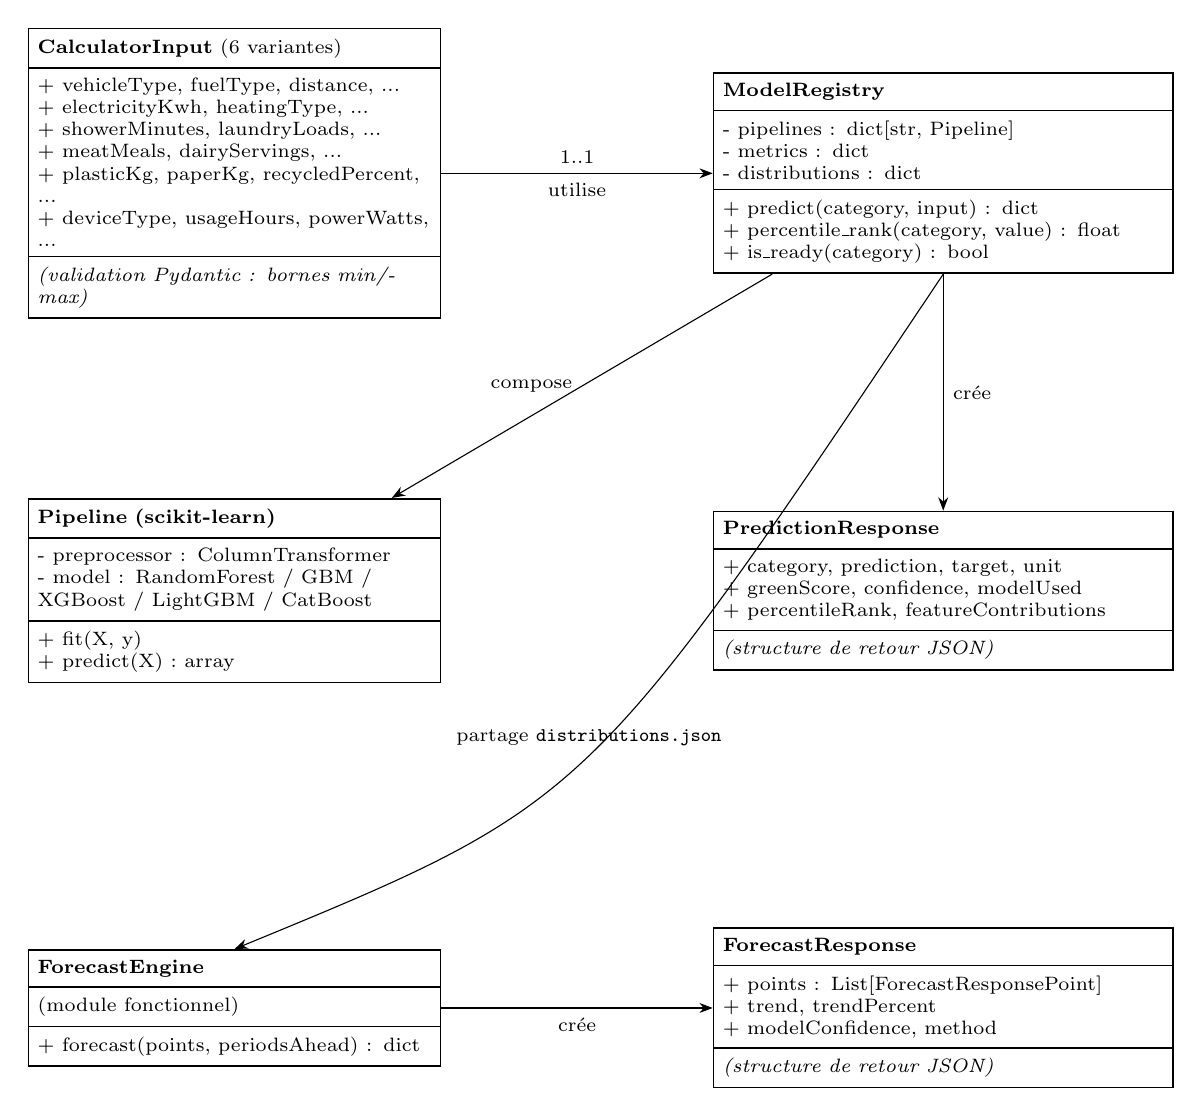
\begin{tikzpicture}[>=Stealth, font=\scriptsize]

\tikzset{
  cls/.style={draw, rectangle split, rectangle split parts=3, text width=5cm, align=left, line width=0.6pt},
}

\node[cls] (input) at (0,0) {
  \centering\textbf{CalculatorInput} \scriptsize(6 variantes)
  \nodepart{second}
  + vehicleType, fuelType, distance, ... \newline
  + electricityKwh, heatingType, ... \newline
  + showerMinutes, laundryLoads, ... \newline
  + meatMeals, dairyServings, ... \newline
  + plasticKg, paperKg, recycledPercent, ... \newline
  + deviceType, usageHours, powerWatts, ...
  \nodepart{third}
  \textit{(validation Pydantic~: bornes min/max)}
};

\node[cls, text width=5.6cm] (registry) at (9,0) {
  \centering\textbf{ModelRegistry}
  \nodepart{second}
  - pipelines~: dict[str, Pipeline] \newline
  - metrics~: dict \newline
  - distributions~: dict
  \nodepart{third}
  + predict(category, input)~: dict \newline
  + percentile\_rank(category, value)~: float \newline
  + is\_ready(category)~: bool
};

\node[cls, text width=5.6cm] (response) at (9,-5.3) {
  \centering\textbf{PredictionResponse}
  \nodepart{second}
  + category, prediction, target, unit \newline
  + greenScore, confidence, modelUsed \newline
  + percentileRank, featureContributions
  \nodepart{third}
  \textit{(structure de retour JSON)}
};

\node[cls, text width=5cm] (pipeline) at (0,-5.3) {
  \centering\textbf{Pipeline (scikit-learn)}
  \nodepart{second}
  - preprocessor~: ColumnTransformer \newline
  - model~: RandomForest / GBM / \newline~~~XGBoost / LightGBM / CatBoost
  \nodepart{third}
  + fit(X, y) \newline
  + predict(X)~: array
};

\node[cls, text width=5cm] (forecast) at (0,-10.6) {
  \centering\textbf{ForecastEngine}
  \nodepart{second}
  (module fonctionnel)
  \nodepart{third}
  + forecast(points, periodsAhead)~: dict
};

\node[cls, text width=5.6cm] (forecastresp) at (9,-10.6) {
  \centering\textbf{ForecastResponse}
  \nodepart{second}
  + points~: List[ForecastResponsePoint] \newline
  + trend, trendPercent \newline
  + modelConfidence, method
  \nodepart{third}
  \textit{(structure de retour JSON)}
};

\draw[->] (input) -- node[above, font=\scriptsize] {1..1} node[below, font=\scriptsize]{utilise} (registry);
\draw[->] (registry) -- node[left, font=\scriptsize] {compose} (pipeline);
\draw[->] (registry) -- node[right, font=\scriptsize] {crée} (response);
\draw[->] (forecast) -- node[below, font=\scriptsize] {crée} (forecastresp);
\draw[->] (registry.south) .. controls (4.5,-8) .. (forecast.north) node[midway, above, font=\scriptsize]{partage \texttt{distributions.json}};

\end{tikzpicture}
}
\caption{Diagramme de classes -- domaine du micro-service Machine Learning}
\label{fig:classes}
\end{figure}

\subsection{Diagramme de séquence}

La figure~\ref{fig:sequence} illustre le scénario nominal \textit{« un utilisateur effectue un calcul d'empreinte carbone »}, depuis la saisie du formulaire jusqu'à l'enregistrement du résultat dans l'historique.

\begin{figure}[H]
\centering
\resizebox{\textwidth}{!}{
\begin{tikzpicture}[>=Stealth, font=\scriptsize]

\def\lifelines{Utilisateur/0, Frontend (React)/3.2, API FastAPI/7, ModelRegistry/10.6, Supabase/14}

\foreach \name/\x in \lifelines {
    \node[draw, fill=isiBlue!15, minimum width=2.6cm, minimum height=0.8cm, align=center, line width=0.6pt] (head-\x) at (\x,0) {\name};
    \draw[dashed] (\x,0) -- (\x,-13.5);
}

% Messages (from-x, to-x, y, label, style)
\draw[->] (0,-1) -- (3.2,-1) node[midway, above, font=\scriptsize]{1. Saisit le formulaire};
\draw[->] (3.2,-1.9) -- (3.4,-1.9) node[midway, above, font=\scriptsize, xshift=1.4cm]{2. Valide localement (bornes)};
\draw[->] (3.2,-2.8) -- (7,-2.8) node[midway, above, font=\scriptsize]{3. POST /api/predict/\{category\}};
\draw[->] (7,-3.7) -- (7.2,-3.7) node[midway, above, font=\scriptsize, xshift=1.9cm]{4. Valide le schéma (Pydantic)};
\draw[->] (7,-4.6) -- (10.6,-4.6) node[midway, above, font=\scriptsize]{5. predict(category, data)};
\draw[->] (10.6,-5.5) -- (10.8,-5.5) node[midway, above, font=\scriptsize, xshift=1.9cm]{6. pipeline.predict(row)};
\draw[->, dashed] (10.6,-6.4) -- (7,-6.4) node[midway, above, font=\scriptsize]{7. prediction, greenScore, ...};
\draw[->, dashed] (7,-7.3) -- (3.2,-7.3) node[midway, above, font=\scriptsize]{8. 200 OK (JSON)};
\draw[->] (3.2,-8.2) -- (3.4,-8.2) node[midway, above, font=\scriptsize, xshift=1.4cm]{9. Affiche le résultat};
\draw[->] (3.2,-9.4) -- (14,-9.4) node[midway, above, font=\scriptsize]{10. insert analyses (inputs, outputs, co2e)};
\draw[->] (14,-10.3) -- (14.2,-10.3) node[midway, above, font=\scriptsize, xshift=2cm]{11. Vérifie RLS (auth.uid() = user\_id)};
\draw[->, dashed] (14,-11.2) -- (3.2,-11.2) node[midway, above, font=\scriptsize]{12. Confirmation};
\draw[->] (3.2,-12.4) -- (0.3,-12.4) node[midway, above, font=\scriptsize]{13. Affiche la confirmation};

\end{tikzpicture}
}
\caption{Diagramme de séquence -- réalisation d'un calcul d'empreinte}
\label{fig:sequence}
\end{figure}

\subsection{Diagramme d'activité}

La figure~\ref{fig:activite} détaille le déroulement du pipeline d'entraînement des modèles de Machine Learning (script \texttt{train.py}), exécuté hors ligne pour chacune des six catégories.

\begin{figure}[H]
\centering
\begin{tikzpicture}[>=Stealth, font=\scriptsize, node distance=0.55cm and 1cm]

\tikzset{
  act/.style={draw, rounded corners=3pt, fill=isiBlue!10, minimum width=6.4cm, minimum height=0.9cm, align=center, line width=0.6pt},
  startstop/.style={circle, draw, fill=black, minimum size=0.28cm},
  endstop/.style={circle, draw, minimum size=0.4cm}
}

\node[startstop] (start) at (0,0) {};
\node[act] (a1) at (0,-1.1) {Charger le jeu de données brut réel (CSV public)};
\node[act] (a2) at (0,-2.3) {Nettoyer et filtrer les données};
\node[act] (a3) at (0,-3.5) {Construire la variable cible (formule physique documentée + bruit réaliste)};
\node[act] (a4) at (0,-4.9) {Encoder les variables catégorielles (\textit{One-Hot Encoding})};
\node[act] (a5) at (0,-6.1) {Diviser en jeu d'entraînement (80\%) et de test (20\%)};
\node[act, minimum height=1.3cm] (a6) at (0,-7.7) {Entraîner et évaluer les 5 algorithmes\\(Random Forest, Gradient Boosting, XGBoost, LightGBM, CatBoost)};
\node[act] (a7) at (0,-9.3) {Sélectionner le modèle au R\textsuperscript{2} le plus élevé};
\node[act] (a8) at (0,-10.5) {Sauvegarder le pipeline retenu (\texttt{.joblib})};
\node[act] (a9) at (0,-11.7) {Générer \texttt{metrics.json} et \texttt{distributions.json}};
\node[endstop] (end) at (0,-12.7) {};
\node[circle, draw, fill=black, minimum size=0.18cm] at (end) {};

\draw[->] (start) -- (a1);
\draw[->] (a1) -- (a2);
\draw[->] (a2) -- (a3);
\draw[->] (a3) -- (a4);
\draw[->] (a4) -- (a5);
\draw[->] (a5) -- (a6);
\draw[->] (a6) -- (a7);
\draw[->] (a7) -- (a8);
\draw[->] (a8) -- (a9);
\draw[->] (a9) -- (end);

\node[font=\scriptsize, align=left, text width=4.5cm] at (5.2,-7.7) {\textit{Répété pour chacune des 6 catégories~: carbon, energy, electronics, water, food, waste}};
\draw[->, dashed] (3.3,-7.7) -- (5.2,-7.7);

\end{tikzpicture}
\caption{Diagramme d'activité -- pipeline d'entraînement des modèles}
\label{fig:activite}
\end{figure}

\subsection{Diagramme de déploiement}

La figure~\ref{fig:deploiement} présente l'architecture de déploiement telle que définie dans le fichier \texttt{docker-compose.yml}~: deux conteneurs Docker orchestrés (frontend et micro-service ML), communiquant avec la plateforme Supabase hébergée dans le cloud.

\begin{figure}[H]
\centering
\resizebox{0.92\textwidth}{!}{
\begin{tikzpicture}[>=Stealth, font=\scriptsize]

\tikzset{
  node3d/.style={draw, rounded corners=2pt, minimum width=5cm, minimum height=1.6cm, align=center, line width=0.7pt},
  stereo/.style={font=\scriptsize\itshape}
}

\node[node3d, fill=isiBlue!8] (browser) at (0,4) {\stereo{«device»}\\\textbf{Poste client}\\Navigateur Web};

\node[node3d, fill=isiBlue!20, minimum height=2.1cm] (nginx) at (-4.5,0) {
  \stereo{«conteneur Docker»}\\
  \textbf{frontend}\\
  \footnotesize nginx:1.27-alpine\\
  Port 8080 → 80\\
  Artefact~: \texttt{dist/} (build React)
};

\node[node3d, fill=isiBlue!20, minimum height=2.1cm] (mlnode) at (4.5,0) {
  \stereo{«conteneur Docker»}\\
  \textbf{ml-service}\\
  \footnotesize python:3.x + FastAPI + uvicorn\\
  Port 8000\\
  Artefacts~: \texttt{*\_model.joblib}
};

\node[node3d, fill=isiBlue!35, minimum height=1.9cm] (supa) at (0,-4) {
  \stereo{«service Cloud»}\\
  \textbf{Supabase}\\
  \footnotesize PostgreSQL + Auth + RLS
};

\draw[<->] (browser) -- (nginx) node[midway, left, font=\scriptsize]{HTTP :8080};
\draw[<->] (browser) -- (mlnode) node[midway, right, font=\scriptsize]{REST/JSON :8000};
\draw[<->] (nginx) -- (supa) node[midway, below, sloped, font=\scriptsize]{HTTPS (SDK)};
\draw[<->, dashed] (nginx) -- (mlnode) node[midway, above, font=\scriptsize]{depends\_on: healthy};

\end{tikzpicture}
}
\caption{Diagramme de déploiement -- environnement Docker Compose}
\label{fig:deploiement}
\end{figure}

\section{Base de données}

GREENLY utilise une base de données PostgreSQL hébergée sur Supabase. Le schéma repose sur une table principale, \texttt{analyses}, reliée à la table système \texttt{auth.users} gérée nativement par Supabase pour l'authentification. La figure~\ref{fig:erd} présente le diagramme entité-association correspondant.

\begin{figure}[H]
\centering
\begin{tikzpicture}[>=Stealth, font=\scriptsize]

\node[draw, rectangle split, rectangle split parts=2, text width=4.6cm, align=left, line width=0.7pt, fill=isiBlue!15] (users) at (0,0) {
  \centering\textbf{auth.users} \scriptsize(géré par Supabase)
  \nodepart{second}
  \underline{id}~: uuid (PK)\\
  email~: text\\
  created\_at~: timestamptz
};

\node[draw, rectangle split, rectangle split parts=2, text width=6.2cm, align=left, line width=0.7pt, fill=isiBlue!8] (analyses) at (9,0) {
  \centering\textbf{analyses}
  \nodepart{second}
  \underline{id}~: uuid (PK)\\
  user\_id~: uuid (FK → auth.users.id)\\
  category~: text \textit{(check~: 6 valeurs)}\\
  inputs~: jsonb\\
  outputs~: jsonb\\
  ai\_recommendation~: text\\
  green\_score~: integer\\
  co2e~: numeric\\
  notes~: text\\
  created\_at~: timestamptz\\
  updated\_at~: timestamptz
};

\draw[-] (users.east) -- (analyses.west) node[midway, above, font=\scriptsize]{1} node[near end, above, font=\scriptsize]{N};

\end{tikzpicture}
\caption{Diagramme entité-association -- schéma de la base de données}
\label{fig:erd}
\end{figure}

Un utilisateur (\texttt{auth.users}) peut posséder de zéro à plusieurs analyses (\texttt{analyses}), relation modélisée par la clé étrangère \texttt{user\_id}. Trois index sont définis pour optimiser les requêtes les plus fréquentes~: sur \texttt{user\_id} (filtrage par utilisateur), sur \texttt{created\_at} (tri chronologique de l'historique) et sur \texttt{category} (filtrage par type de calculateur). La sécurité d'accès est assurée par quatre politiques \textbf{RLS} (\textit{Row Level Security}) -- une par opération CRUD -- garantissant qu'un utilisateur authentifié ne peut lire, insérer, modifier ou supprimer que les lignes dont il est propriétaire~:

\begin{lstlisting}
CREATE POLICY "select_own_analyses" ON analyses FOR SELECT
  TO authenticated USING (auth.uid() = user_id);
\end{lstlisting}

\section{Architecture Frontend / Backend}

\subsection{Frontend}
L'interface utilisateur est développée en \textbf{React 18} avec \textbf{TypeScript}, à l'aide de l'outil de build \textbf{Vite}. La mise en forme repose sur \textbf{Tailwind CSS} combiné aux composants accessibles \textbf{Radix UI} (via la bibliothèque de composants shadcn/ui). Le routage est assuré par \texttt{react-router-dom}, les formulaires par \texttt{react-hook-form} couplé à des schémas de validation \texttt{zod}, et les visualisations par la bibliothèque \texttt{recharts}. L'organisation du code suit une architecture en couches~:

\begin{itemize}[label=\textbullet,font=\normalsize]
    \item \texttt{pages/} -- les vues de l'application (landing, authentification, calculateurs, tableaux de bord)~;
    \item \texttt{services/} -- la couche d'accès aux données externes (\texttt{mlService.ts} pour l'API ML, \texttt{analysisService.ts} pour Supabase, \texttt{pdfReportService.ts} pour l'export PDF)~;
    \item \texttt{lib/} -- la logique métier pure (\texttt{calculators.ts}, formatage, configuration des calculateurs)~;
    \item \texttt{hooks/} et \texttt{contexts/} -- la gestion d'état partagé (authentification, thème, historique des analyses)~;
    \item \texttt{components/} -- les composants d'interface réutilisables.
\end{itemize}

\subsection{Backend -- micro-service Machine Learning}
Le micro-service est développé en Python avec \textbf{FastAPI}, choisi pour sa validation native des données via \textbf{Pydantic}, ses performances asynchrones et la génération automatique d'une documentation interactive (OpenAPI/Swagger). Il est structuré en trois modules principaux~: \texttt{routers/} (points d'entrée REST), \texttt{registry.py} (chargement et orchestration des modèles), et \texttt{schemas.py} (contrats de données d'entrée/sortie).

\subsection{Backend -- persistance}
La persistance et l'authentification sont déléguées à \textbf{Supabase}, une plateforme \textit{Backend-as-a-Service} bâtie sur PostgreSQL. Ce choix permet de bénéficier d'une authentification robuste, d'une sécurité déclarative (RLS) et d'un SDK JavaScript directement intégrable côté client, sans développer de backend applicatif dédié à la gestion des utilisateurs.

\section{Description des modules}

Le tableau~\ref{tab:modules} résume les principaux modules du micro-service Machine Learning et leur responsabilité.

\begin{table}[H]
\centering
\caption{Description des modules du micro-service ML}
\label{tab:modules}
\begin{tabular}{|p{3.6cm}|p{9.5cm}|}
\hline
\rowcolor{isiBlue!15}
\textbf{Module} & \textbf{Responsabilité} \\
\hline
\texttt{scripts/download\_datasets.py} & Télécharge les jeux de données publics bruts (EPA, UCI, Our World in Data). \\ \hline
\texttt{scripts/prepare\_datasets.py} & Nettoie les données brutes et construit les variables cibles (labels) d'entraînement selon des formules physiques documentées. \\ \hline
\texttt{scripts/train.py} & Entraîne et compare 5 algorithmes par catégorie, sélectionne et sauvegarde le meilleur modèle. \\ \hline
\texttt{app/schemas.py} & Définit les schémas Pydantic de validation des requêtes et réponses de l'API. \\ \hline
\texttt{app/registry.py} & Charge les pipelines entraînés en mémoire et expose la fonction de prédiction. \\ \hline
\texttt{app/forecasting.py} & Calcule la tendance statistique (régression linéaire) sur l'historique d'un utilisateur. \\ \hline
\texttt{app/routers/predict.py} & Expose les routes \texttt{POST /api/predict/\{category\}}. \\ \hline
\texttt{app/routers/analytics.py} & Expose les routes de métriques de modèles et de prévision. \\ \hline
\texttt{app/main.py} & Point d'entrée FastAPI~: assemblage des routers, configuration CORS. \\ \hline
\end{tabular}
\end{table}

\section{Dataset}

Contrairement à une approche à formule fixe, GREENLY fonde ses prédictions sur l'entraînement de modèles supervisés. Or, il n'existe pas de jeu de données public unique reliant directement des habitudes de consommation individuelles à une empreinte carbone mesurée. Une approche \textbf{hybride} a donc été retenue~: pour chaque catégorie, la relation entre les variables d'entrée et la valeur cible est ancrée dans des données publiques réelles et documentées, complétées -- lorsque nécessaire -- par une simulation de distributions d'usage réalistes.

Le tableau~\ref{tab:datasets} présente, pour chaque catégorie, la source réelle utilisée et la nature du jeu de données d'entraînement obtenu.

\begin{table}[H]
\centering
\caption{Sources de données par catégorie}
\label{tab:datasets}
\begin{tabular}{|p{2.1cm}|p{4.6cm}|p{2cm}|p{4.4cm}|}
\hline
\rowcolor{isiBlue!15}
\textbf{Catégorie} & \textbf{Source réelle} & \textbf{Taille} & \textbf{Nature} \\
\hline
Transport & EPA \texttt{fueleconomy.gov} -- \texttt{vehicles.csv} (émissions mesurées réelles) \cite{epaVehicles} & 67~189 lignes & Réelle + distances simulées \\ \hline
Énergie & UCI \textit{Appliances Energy Prediction} \cite{candanedo2017} (mesures de capteurs réelles) & 12~000 lignes & Réelle + mise à l'échelle par foyer \\ \hline
Électronique & Constantes EPA ENERGY STAR / DOE (puissances typiques) \cite{energyStar} & 8~000 lignes & Simulation à partir de constantes réelles \\ \hline
Eau & Constantes EPA WaterSense / USGS (débits typiques) \cite{waterSense} & 8~000 lignes & Simulation à partir de constantes réelles \\ \hline
Alimentation & Our World in Data / Poore \& Nemecek (2018) \cite{poore2018} (émissions réelles par aliment) & 8~000 lignes & Réelle (intensités) + repas simulés \\ \hline
Déchets & Our World in Data -- taux de collecte des déchets \cite{owidWaste} & 8~000 lignes & Réelle (taux de recyclage) + composition simulée \\ \hline
\end{tabular}
\end{table}

Chaque constante physique utilisée (facteur d'émission du réseau électrique, intensité carbone d'un type de chauffage, débit d'une douche économe, etc.) est documentée dans le code source et rattachée à sa source officielle, garantissant la traçabilité scientifique du système -- un point que le chapitre~1 identifiait comme une lacune des outils existants.

\section{Prétraitement}

Le prétraitement des données se déroule en deux temps~: la construction du jeu de données d'entraînement (variable cible), puis sa préparation pour l'algorithme d'apprentissage.

\subsection{Construction de la variable cible}
Pour la catégorie Transport, à titre d'exemple, l'émission mesurée par l'EPA (en grammes de CO2 par mile, valeur réelle) est convertie en kilogrammes par kilomètre, puis combinée à une distance simulée et à un facteur correctif « conditions réelles vs laboratoire » (écart documenté par l'EPA et l'ICCT, de l'ordre de 10 à 25\,\%)~:

\begin{lstlisting}[language=Python]
co2_per_km = (co2TailpipeGpm / 1000) / 1.60934
real_world_factor = np.clip(RNG.normal(1.15, 0.08), 0.9, 1.45)
co2e_kg = co2_per_km * distance_km * real_world_factor
\end{lstlisting}

\subsection{Encodage et découpage}
Les variables catégorielles (par exemple \texttt{vehicleType}, \texttt{fuelType}) sont encodées par \textbf{One-Hot Encoding}, tandis que les variables numériques sont conservées telles quelles (les modèles à base d'arbres de décision ne nécessitant pas de normalisation). Le jeu de données est ensuite scindé en un ensemble d'entraînement (80\,\%) et un ensemble de test (20\,\%), ce dernier n'étant jamais utilisé pendant l'apprentissage afin de garantir une évaluation non biaisée~:

\begin{lstlisting}[language=Python]
preprocessor = ColumnTransformer([
    ("cat", OneHotEncoder(handle_unknown="ignore"), categorical),
    ("num", "passthrough", numeric),
])
X_train, X_test, y_train, y_test = train_test_split(
    X, y, test_size=0.2, random_state=42
)
\end{lstlisting}

\section{Entraînement des modèles de Machine Learning}

Pour chacune des six catégories, cinq algorithmes de régression supervisée sont entraînés et comparés automatiquement~:

\begin{itemize}[label=\textbullet,font=\normalsize]
    \item \textbf{Random Forest} \cite{breiman2001}~: forêt de 300 arbres de décision (profondeur maximale~14), moyennant leurs prédictions individuelles.
    \item \textbf{Gradient Boosting}~: 300 arbres construits séquentiellement, chacun corrigeant l'erreur résiduelle du précédent (taux d'apprentissage~0,05).
    \item \textbf{XGBoost} \cite{chen2016}~: implémentation optimisée du \textit{gradient boosting} (400 arbres, profondeur~6).
    \item \textbf{LightGBM} \cite{ke2017}~: variante de \textit{gradient boosting} à croissance par feuille, optimisée pour la vitesse (400 arbres).
    \item \textbf{CatBoost} \cite{prokhorenkova2018}~: \textit{gradient boosting} avec un traitement natif optimisé des variables catégorielles (400 itérations, profondeur~6).
\end{itemize}

Ces cinq algorithmes reposent tous sur le principe des \textbf{ensembles d'arbres de décision}, particulièrement adaptés aux données tabulaires mixtes (catégorielles et numériques) et capables de modéliser des interactions non linéaires entre variables, contrairement aux formules linéaires fixes utilisées par les outils concurrents (voir chapitre~1). Le meilleur algorithme est sélectionné automatiquement selon le coefficient de détermination R\textsuperscript{2} obtenu sur le jeu de test~:

\begin{lstlisting}[language=Python]
for algo_name, make_model in ALGORITHMS.items():
    pipeline = Pipeline([("prep", preprocessor), ("model", make_model())])
    pipeline.fit(X_train, y_train)
    preds = pipeline.predict(X_test)
    r2 = r2_score(y_test, preds)
    if r2 > best_score:
        best_name, best_score, best_pipeline = algo_name, r2, pipeline
joblib.dump(best_pipeline, MODELS / f"{category}_model.joblib")
\end{lstlisting}

\section{Évaluation}

Trois métriques standard de régression sont utilisées pour évaluer chaque modèle sur le jeu de test (données jamais vues pendant l'entraînement)~:

\begin{itemize}[label=\textbullet,font=\normalsize]
    \item \textbf{MAE} (\textit{Mean Absolute Error})~: erreur absolue moyenne, dans l'unité de la variable cible~;
    \item \textbf{RMSE} (\textit{Root Mean Squared Error})~: pénalise davantage les grosses erreurs~;
    \item \textbf{R\textsuperscript{2}} (coefficient de détermination)~: proportion de la variance de la cible expliquée par le modèle (1 = prédiction parfaite).
\end{itemize}

Le tableau~\ref{tab:comparaison-algos} présente la comparaison complète des 5 algorithmes pour la catégorie Transport, obtenue lors de l'exécution réelle du pipeline d'entraînement.

\begin{table}[H]
\centering
\caption{Comparaison des 5 algorithmes -- catégorie Transport (67~189 trajets, 20\,\% test)}
\label{tab:comparaison-algos}
\begin{tabular}{|l|c|c|c|}
\hline
\rowcolor{isiBlue!15}
\textbf{Algorithme} & \textbf{MAE (kg)} & \textbf{RMSE (kg)} & \textbf{R\textsuperscript{2}} \\
\hline
\textbf{Gradient Boosting (retenu)} & \textbf{1,878} & \textbf{4,218} & \textbf{0,9824} \\ \hline
Random Forest & 1,902 & 4,629 & 0,9788 \\ \hline
LightGBM & 1,980 & 6,561 & 0,9574 \\ \hline
CatBoost & 2,033 & 6,854 & 0,9535 \\ \hline
XGBoost & 2,017 & 7,058 & 0,9507 \\ \hline
\end{tabular}
\end{table}

Le tableau~\ref{tab:resultats-globaux} synthétise le modèle finalement retenu pour chacune des six catégories du système.

\begin{table}[H]
\centering
\caption{Modèle retenu et performance par catégorie (données réelles \texttt{metrics.json})}
\label{tab:resultats-globaux}
\begin{tabular}{|l|l|c|c|c|}
\hline
\rowcolor{isiBlue!15}
\textbf{Catégorie} & \textbf{Algorithme retenu} & \textbf{R\textsuperscript{2}} & \textbf{MAE} & \textbf{RMSE} \\
\hline
Énergie & CatBoost & 0,9993 & 1,808 & 2,550 \\ \hline
Déchets & CatBoost & 0,9993 & 0,052 & 0,104 \\ \hline
Électronique & CatBoost & 0,9875 & 0,036 & 0,061 \\ \hline
Transport & Gradient Boosting & 0,9824 & 1,878 & 4,218 \\ \hline
Eau & CatBoost & 0,7820 & 57,76 & 77,38 \\ \hline
Alimentation & CatBoost & 0,5667 & 11,85 & 15,76 \\ \hline
\end{tabular}
\end{table}

L'analyse de ces résultats appelle une remarque importante~: la précision varie sensiblement selon la catégorie. Les catégories Énergie, Déchets et Électronique, où la cible dépend directement de facteurs physiques appliqués aux variables observées, atteignent une précision quasi parfaite. À l'inverse, les catégories Eau et surtout Alimentation intègrent, lors de la construction du jeu d'entraînement, des facteurs de variation aléatoire (par exemple la composition exacte du régime alimentaire d'un utilisateur) qui ne sont \textbf{pas} observables dans les variables d'entrée fournies au modèle~; ce bruit non observable constitue un plafond théorique de précision, quel que soit l'algorithme utilisé -- et non un défaut de modélisation.

\section{Intégration des modèles IA dans l'application}

Les pipelines entraînés (prétraitement + modèle, sérialisés au format \texttt{.joblib}) sont chargés une seule fois, au démarrage du micro-service, par la classe \texttt{ModelRegistry} (voir diagramme de classes, figure~\ref{fig:classes}), qui les conserve en mémoire pour garantir des temps de réponse de l'ordre de la dizaine de millisecondes. Chaque requête de prédiction déclenche la séquence suivante (détaillée dans le diagramme de séquence, figure~\ref{fig:sequence})~:

\begin{enumerate}
    \item validation du corps de la requête par un schéma Pydantic dédié à la catégorie~;
    \item construction d'une ligne de données au format attendu par le pipeline~;
    \item appel de \texttt{pipeline.predict()}, qui applique successivement le prétraitement (encodage) puis le modèle entraîné~;
    \item calcul du \textit{Green Score} par positionnement percentile de la prédiction dans la distribution des valeurs observées à l'entraînement (\texttt{distributions.json})~;
    \item retour d'une réponse structurée incluant la prédiction, le score, le niveau de confiance (R\textsuperscript{2} du modèle) et l'importance des variables.
\end{enumerate}

Ce découplage entre entraînement (hors ligne, via \texttt{scripts/train.py}) et inférence (en ligne, via l'API FastAPI) permet de ré-entraîner ou d'ajouter de nouveaux algorithmes sans jamais interrompre le service applicatif.

\section*{Conclusion}
Ce chapitre a détaillé la conception et la réalisation du volet Intelligence Artificielle de GREENLY~: de l'architecture logicielle globale jusqu'à l'intégration effective des modèles entraînés dans l'application, en passant par la constitution rigoureuse des jeux de données, leur prétraitement et l'évaluation comparative de cinq algorithmes d'apprentissage supervisé. Les résultats obtenus, avec un coefficient R\textsuperscript{2} atteignant 0,999 pour certaines catégories, démontrent la viabilité de l'approche. Le chapitre suivant présente le second volet du projet~: le module de Business Intelligence et de prévision, qui exploite ces modèles pour offrir à l'utilisateur un suivi analytique de son impact environnemental.

        \clearpage
        
        \chapter{Volet Business Intelligence et Prévision}

\section*{Introduction}
Au-delà de la prédiction ponctuelle d'une empreinte environnementale, GREENLY vise à donner à l'utilisateur une vision analytique et évolutive de son impact. Ce quatrième chapitre présente le second grand volet du projet~: le module de \textbf{Business Intelligence} (BI), qui transforme l'historique des analyses individuelles en indicateurs, tableaux de bord et prévisions exploitables. Nous y détaillons l'architecture décisionnelle retenue, les indicateurs clés de performance calculés, les tableaux de bord et visualisations développés, le module de prévision statistique, ainsi que le système de recommandations personnalisées.

\section{Architecture BI}

Contrairement à une architecture décisionnelle classique reposant sur un entrepôt de données (\textit{data warehouse}) séparé et des traitements ETL périodiques, GREENLY adopte une architecture BI \textbf{légère et temps réel}, adaptée à l'échelle d'un historique individuel~:

\begin{itemize}[label=\textbullet,font=\normalsize]
    \item la table \texttt{analyses} de la base Supabase joue le rôle de \textbf{table de faits}~: chaque ligne représente un événement de mesure (une analyse), avec ses dimensions (catégorie, date) et ses mesures (\texttt{co2e}, \texttt{green\_score}, contenu JSON \texttt{outputs})~;
    \item l'\textbf{agrégation} (regroupement mensuel, annuel, par catégorie) est calculée \textbf{côté client}, en React, via des fonctions mémoïsées (\texttt{useMemo}) qui recalculent les indicateurs à chaque changement de filtre (période, catégorie) sans requête serveur supplémentaire~;
    \item le \textbf{calcul prédictif} (prévision de tendance) est délégué au micro-service ML via l'endpoint \texttt{POST~/api/forecast}, qui applique une régression statistique sur les points d'historique transmis par le client.
\end{itemize}

Ce choix d'architecture évite la complexité d'un entrepôt de données dédié, injustifiée à l'échelle des volumes traités (historique d'un utilisateur individuel), tout en conservant la réactivité nécessaire à une expérience de tableau de bord interactif.

\section{KPIs}

Le tableau~\ref{tab:kpis} présente les indicateurs clés de performance (\textit{Key Performance Indicators}) calculés et affichés par la plateforme.

\begin{table}[H]
\centering
\caption{Indicateurs clés de performance (KPI) de GREENLY}
\label{tab:kpis}
\begin{tabular}{|p{3.4cm}|p{6.4cm}|p{3.5cm}|}
\hline
\rowcolor{isiBlue!15}
\textbf{KPI} & \textbf{Définition} & \textbf{Mode de calcul} \\
\hline
Green Score & Score de 0 à 100 situant une analyse par rapport à la distribution des valeurs observées à l'entraînement. & $100 - \text{percentile}$ (voir chapitre~3) \\ \hline
CO2e total & Somme des émissions de CO2 équivalent sur la période et les catégories sélectionnées. & $\sum \texttt{co2e}$ \\ \hline
Consommation d'eau & Somme des litres d'eau calculés sur la période sélectionnée. & $\sum \texttt{waterLiters}$ \\ \hline
Consommation d'énergie & Somme des kWh calculés (énergie domestique + électronique). & $\sum \texttt{energyKwh}$ \\ \hline
Score moyen & Moyenne des \textit{Green Scores} sur la période/catégorie sélectionnée. & $\overline{\texttt{green\_score}}$ \\ \hline
Arbres nécessaires & Nombre d'arbres qu'il faudrait planter pour compenser le CO2e total annuel (1 arbre~$\approx$~21~kg CO2/an). & $\lceil \text{CO2e total} / 21 \rceil$ \\ \hline
Confiance du modèle & Fiabilité du modèle de prédiction de la catégorie active, exprimée en \%. & $R^2_{\text{modèle}} \times 100$ \\ \hline
Erreur de prévision (MAE) & Erreur absolue moyenne du modèle sur le jeu de test, affichée pour contextualiser la confiance accordée à une prédiction. & Voir tableau~\ref{tab:resultats-globaux} \\ \hline
\end{tabular}
\end{table}

\section{Tableaux de bord}

GREENLY propose trois tableaux de bord complémentaires, correspondant à trois niveaux de lecture de l'impact environnemental de l'utilisateur~:

\begin{enumerate}
    \item \textbf{Dashboard (vue d'ensemble)}~: page d'accueil de l'espace utilisateur, présentant les KPI principaux, une jauge de score de durabilité, la tendance mensuelle du CO2e, la répartition des analyses par catégorie, ainsi que des \textit{insights} textuels générés automatiquement (comparaison au mois précédent, catégorie la plus suivie).
    \item \textbf{Tableau de bord BI}~: vue analytique avancée avec filtres par période (3, 6, 12 mois, année en cours) et par catégorie, comparaison annuelle, radar de score par catégorie face à un objectif cible, et une synthèse exécutive générée à partir des agrégats réels de l'utilisateur.
    \item \textbf{AI Analytics}~: vue centrée sur les modèles eux-mêmes~: métriques réelles de performance par catégorie, comparaison des 5 algorithmes, importance des variables, prévision de tendance et recommandations dérivées.
\end{enumerate}

\section{Visualisations}

L'ensemble des visualisations est développé avec la bibliothèque \textbf{Recharts} (React), permettant des graphiques interactifs (infobulles, légendes, mise en évidence au survol) directement intégrés à l'interface. Six familles de représentations graphiques sont utilisées~: graphiques en aires (tendance temporelle), histogrammes (comparaison catégorielle ou annuelle), diagrammes circulaires (répartition), diagrammes radar (score multi-catégoriel face à un objectif), courbes (évolution du score) et graphiques composés (prévision avec intervalle de confiance).

La figure~\ref{fig:bi-r2} présente une donnée réelle du projet~: la précision (R\textsuperscript{2}) du modèle finalement retenu pour chacune des six catégories, telle qu'exposée par l'API \texttt{GET~/api/models/metrics} et affichée sur la page AI Analytics.

\begin{figure}[H]
\centering
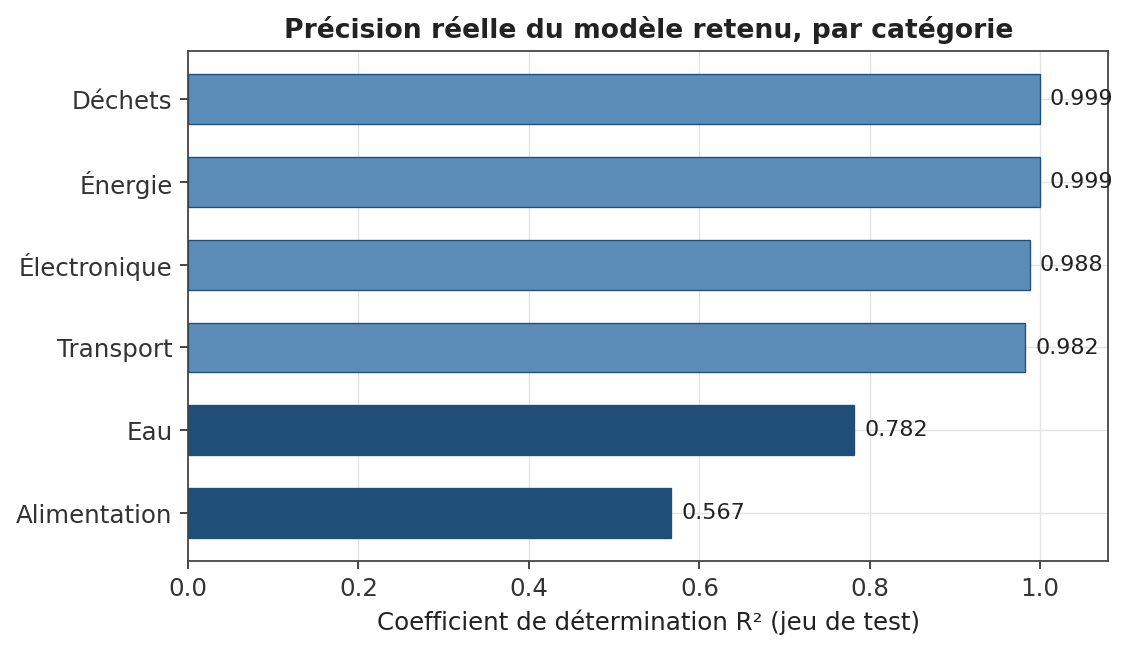
\includegraphics[width=0.82\textwidth]{bi-r2-par-categorie}
\caption{Précision réelle (R\textsuperscript{2}) du modèle retenu par catégorie (donnée réelle \texttt{metrics.json})}
\label{fig:bi-r2}
\end{figure}

Les figures~\ref{fig:bi-tendance} et \ref{fig:bi-repartition} illustrent, à partir de données d'exemple (l'application ne disposant pas encore d'historique utilisateur en production au moment de la rédaction de ce rapport), le rendu des deux graphiques principaux du tableau de bord BI~: la tendance mensuelle multi-indicateurs et la répartition des analyses par catégorie.

\begin{figure}[H]
\centering
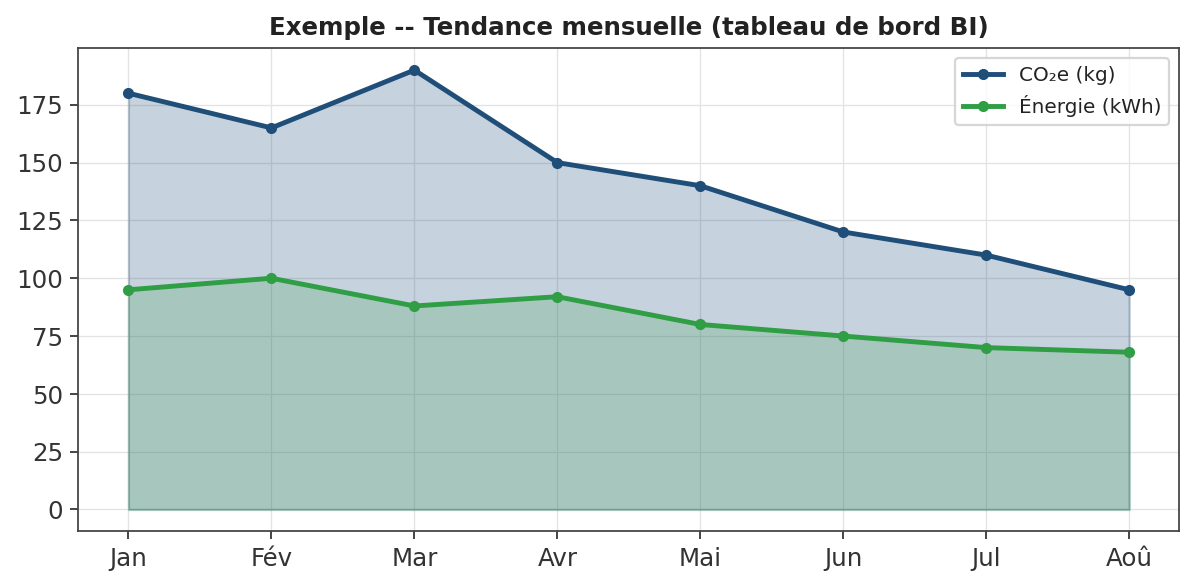
\includegraphics[width=0.85\textwidth]{bi-tendance-mensuelle}
\caption{Exemple de rendu -- tendance mensuelle CO2e / énergie (données d'illustration)}
\label{fig:bi-tendance}
\end{figure}

\begin{figure}[H]
\centering
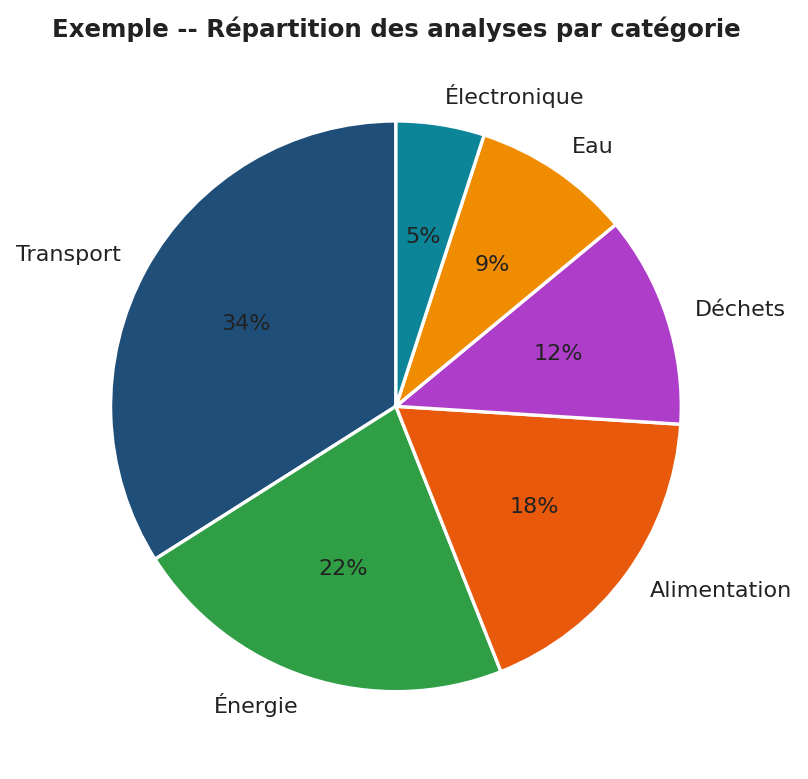
\includegraphics[width=0.6\textwidth]{bi-repartition-categories}
\caption{Exemple de rendu -- répartition des analyses par catégorie (données d'illustration)}
\label{fig:bi-repartition}
\end{figure}

La figure~\ref{fig:bi-radar} illustre le graphique radar comparant, pour chaque catégorie, le score moyen de l'utilisateur à un objectif fixé à 85/100 -- une représentation particulièrement efficace pour identifier en un coup d'œil les catégories prioritaires d'amélioration.

\begin{figure}[H]
\centering
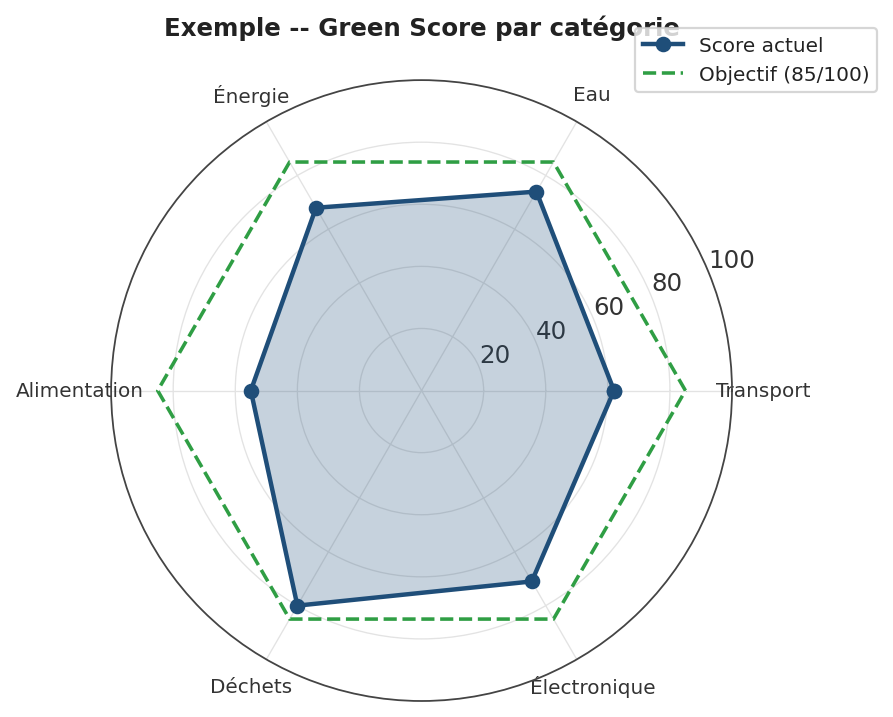
\includegraphics[width=0.55\textwidth]{bi-radar-score}
\caption{Exemple de rendu -- Green Score par catégorie face à l'objectif (données d'illustration)}
\label{fig:bi-radar}
\end{figure}

\section{Prévisions}

Le module de prévision (\texttt{app/forecasting.py}) projette la tendance future d'un utilisateur à partir de son historique réel de \textit{Green Scores} ou de valeurs d'empreinte, catégorie par catégorie. Volontairement, ce module \textbf{n'utilise pas} un modèle de \textit{Machine Learning} complexe ni de saisonnalité simulée~: le service ML n'a pas accès à l'historique complet de l'utilisateur (celui-ci résidant côté Supabase/frontend), et une régression linéaire simple sur les points réellement transmis par le client est jugée plus honnête qu'un modèle sophistiqué appliqué à un historique potentiellement très court.

La méthode ajuste une régression linéaire $y = a x + b$ par la méthode des moindres carrés sur les $n$ points d'historique, puis extrapole sur les périodes futures demandées, avec un intervalle de confiance qui \textbf{s'élargit avec l'horizon de projection}~:

\begin{lstlisting}[language=Python]
slope, intercept = np.polyfit(x, values, 1)
fitted = slope * x + intercept
residual_std = np.std(values - fitted)
...
widen = residual_std * (1 + 0.15 * i)   # incertitude croissante avec l'horizon
predicted = slope * future_x + intercept
\end{lstlisting}

Le niveau de confiance accordé à la prévision (\texttt{modelConfidence}) n'est pas une constante arbitraire~: il combine la qualité de l'ajustement (un pseudo-R\textsuperscript{2} calculé sur les résidus) et la taille de l'échantillon disponible (une prévision fondée sur 2 points est nécessairement moins fiable qu'une prévision fondée sur 12 points)~:

\begin{lstlisting}[language=Python]
r2 = 1 - (np.var(residuals) / np.var(values))
sample_factor = min(1.0, n / 12)
model_confidence = 0.5 * max(0.0, r2) + 0.5 * sample_factor
\end{lstlisting}

La figure~\ref{fig:bi-forecast} présente une exécution \textbf{réelle} de cet algorithme (code non modifié, exécuté tel quel), appliquée à un historique d'exemple de huit mois de CO2e mensuel. La tendance détectée est \textit{décroissante} ($-14{,}4\,\%$ projetés sur les 4 prochains mois), illustrant une situation où l'empreinte de l'utilisateur s'améliore dans le temps.

\begin{figure}[H]
\centering
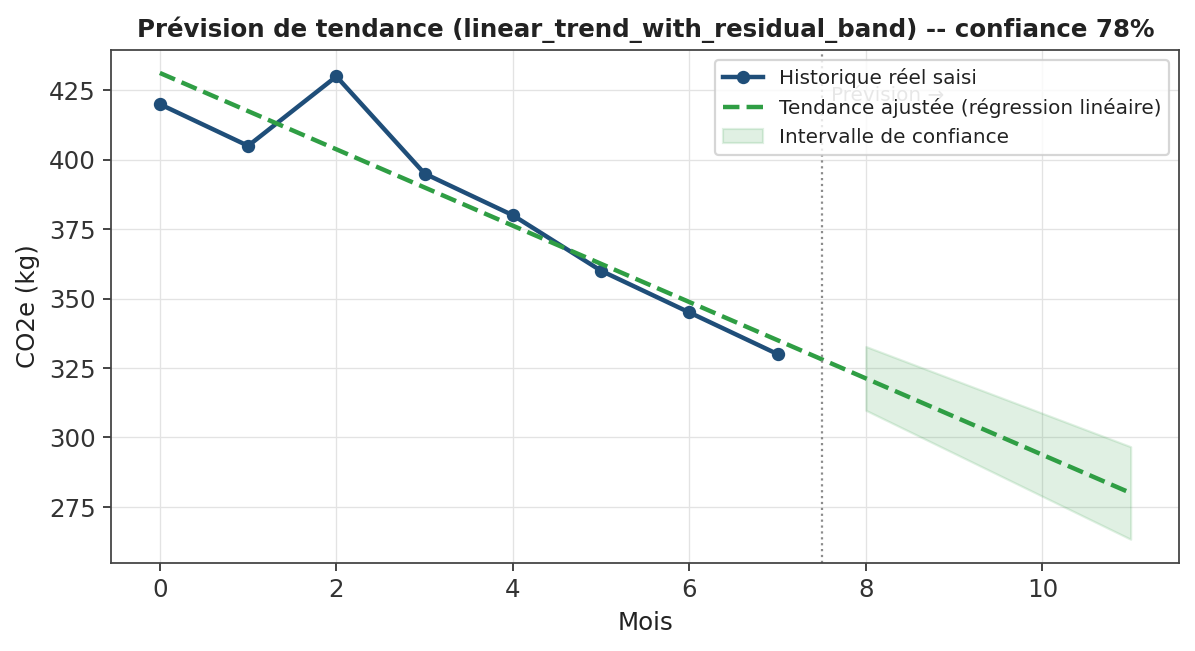
\includegraphics[width=0.85\textwidth]{bi-forecast}
\caption{Prévision de tendance -- exécution réelle de l'algorithme sur un historique d'exemple}
\label{fig:bi-forecast}
\end{figure}

\section{Analyses}

Au-delà des graphiques, le tableau de bord BI génère une \textbf{synthèse analytique automatique} (« AI Executive Summary ») directement calculée à partir des agrégats réels de l'utilisateur, sans recours à un service de génération de texte externe~: la meilleure et la moins bonne catégorie sont déterminées par comparaison des scores moyens, et la tendance globale est établie en comparant la moyenne des scores sur la première et la seconde moitié de la période sélectionnée~:

\begin{lstlisting}[language=Python]
sorted_scores = sorted(scoreByCategory, key=lambda s: -s.current)
best, worst = sorted_scores[0], sorted_scores[-1]
improving = secondHalfAvgScore >= firstHalfAvgScore
\end{lstlisting}

Cette synthèse restitue par exemple des messages tels que \textit{« Votre score moyen s'est amélioré de 6 points sur cette période »} ou \textit{« Transport est votre catégorie la plus performante, avec une moyenne de 82/100 »}, personnalisés à chaque utilisateur et recalculés à chaque changement de filtre.

\section{Recommandations}

Le système de recommandations personnalisées constitue l'un des apports les plus directement liés au volet Intelligence Artificielle du chapitre précédent~: plutôt que d'afficher des conseils génériques identiques pour tous les utilisateurs (limite identifiée chez les solutions concurrentes, chapitre~1), GREENLY exploite l'\textbf{importance réelle des variables} (\textit{feature importance}) calculée par chaque modèle entraîné pour cibler la recommandation la plus pertinente pour la situation spécifique de l'utilisateur~:

\begin{lstlisting}[language=Python]
tips = sorted(feature_importance.items(), key=lambda kv: -kv[1])[:3]
# ex. pour la categorie "carbon" :
# distance (43%) -> "La distance domine votre empreinte -- grouper vos
#                     trajets ou le télétravail change beaucoup la donne."
# fuelType (27%) -> "Le type de carburant est un facteur déterminant --
#                     passer à l'hybride ou à l'électrique réduirait..."
\end{lstlisting}

Chaque recommandation est ainsi accompagnée du poids réel (en \%) que la variable correspondante représente dans les prédictions du modèle pour la catégorie concernée, renforçant la transparence et la crédibilité du conseil donné -- un utilisateur voit explicitement \textit{pourquoi} telle variable lui est signalée, plutôt que de recevoir un conseil non justifié.

\section*{Conclusion}
Ce chapitre a présenté le volet Business Intelligence et prévision de GREENLY~: une architecture décisionnelle légère fondée sur l'agrégation côté client, des indicateurs clés de performance directement dérivés des sorties des modèles de Machine Learning, trois tableaux de bord complémentaires, un module de prévision statistique honnête quant à son incertitude, ainsi qu'un système de recommandations personnalisées fondé sur l'importance réelle des variables. Combiné au volet Intelligence Artificielle détaillé au chapitre~3, ce module de Business Intelligence positionne GREENLY comme une plateforme de suivi environnemental complète, dépassant le simple calculateur ponctuel pour offrir un véritable accompagnement dans la durée. Le chapitre suivant conclut ce rapport en dressant le bilan du travail réalisé et en proposant des perspectives d'évolution.

        \clearpage
        
        \chapter*{Conclusion générale}
\addcontentsline{toc}{chapter}{Conclusion générale}
\markboth{Conclusion générale}{}

Ce rapport a présenté la conception, la réalisation et l'évaluation de \textbf{GREENLY}, une plateforme web intelligente combinant Intelligence Artificielle et Business Intelligence pour le calcul et le suivi de l'empreinte environnementale individuelle. Le point de départ de ce projet était un constat simple~: les calculateurs d'empreinte carbone existants, aussi utiles soient-ils, reposent presque tous sur des formules fixes, ne conservent aucun historique et n'offrent aucune prévision ni recommandation réellement personnalisée.

Pour répondre à cette problématique, un pipeline complet de Machine Learning a été conçu et mis en œuvre~: collecte de données publiques réelles (EPA, UCI, Our World in Data), construction rigoureuse et documentée des variables cibles d'entraînement, comparaison objective de cinq algorithmes de régression supervisée pour six catégories d'usage, et intégration des modèles retenus dans une API de prédiction en temps réel. Les résultats obtenus -- un coefficient de détermination R\textsuperscript{2} atteignant 0,999 pour les catégories Énergie et Déchets, et restant supérieur à 0,98 pour le Transport -- démontrent la pertinence de cette approche par apprentissage automatique par rapport aux formules statiques des solutions concurrentes.

Ce socle prédictif a ensuite été exploité par un module de Business Intelligence complet~: indicateurs clés de performance, trois tableaux de bord complémentaires, visualisations interactives, module de prévision statistique honnête quant à son incertitude, et système de recommandations personnalisées fondé sur l'importance réelle des variables de chaque modèle. L'ensemble repose sur une architecture logicielle moderne et déployable -- interface React/TypeScript, micro-service FastAPI, base de données Supabase sécurisée par des politiques RLS -- conteneurisée via Docker pour une mise en production reproductible.

Sur le plan personnel, ce projet a été l'occasion de mettre en pratique, sur un cas réel de bout en bout, l'ensemble du cycle de vie d'un système de Machine Learning~: de la collecte et de la documentation rigoureuse des données jusqu'au déploiement d'une API de prédiction, en passant par la comparaison méthodique de plusieurs algorithmes. Il a également permis d'expérimenter concrètement l'articulation entre un volet prédictif (Intelligence Artificielle) et un volet analytique et décisionnel (Business Intelligence), deux disciplines trop souvent traitées séparément.

Ce travail présente néanmoins certaines limites, qui ouvrent autant de perspectives d'évolution~:

\begin{itemize}[label=\textbullet,font=\normalsize]
\item les jeux de données d'entraînement des catégories Eau, Électronique et Déchets reposent en partie sur des distributions d'usage simulées, faute de données publiques mesurées à l'échelle du foyer~; l'intégration progressive de données réelles d'utilisateurs (avec leur consentement) permettrait d'affiner encore ces modèles~;
\item les facteurs d'émission utilisés sont actuellement calibrés sur le contexte américain (EPA, DOE)~; une régionalisation des facteurs (mix électrique par pays, notamment tunisien ou européen) constituerait une évolution naturelle du projet~;
\item le module de prévision, volontairement simple (régression linéaire), pourrait être enrichi -- une fois un volume suffisant d'historiques utilisateurs disponible -- par des modèles de séries temporelles plus sophistiqués (SARIMA, Prophet)~;
\item une automatisation du cycle de ré-entraînement (pipeline MLOps avec suivi de dérive des données) renforcerait la fiabilité du système dans la durée.
\end{itemize}

En définitive, GREENLY démontre qu'il est possible de concilier rigueur scientifique (traçabilité des sources et des facteurs d'émission), puissance prédictive (Machine Learning plutôt que formules fixes) et accompagnement utilisateur dans la durée (Business Intelligence et prévision), au sein d'une architecture logicielle moderne et déployable.

        \clearpage
        
        % @author: Stoufa
		% the command `\nocite{*}` is mandatory to avoid the “no \citation commands” error
        % https://tex.stackexchange.com/questions/18045/problem-with-compiling-bibtex-no-citation-commands-error
        %\nocite{*}
        \printbibliography[heading=bibintoc]
        
        \chapter*{Annexes}
\addcontentsline{toc}{chapter}{Annexes}
\markboth{Annexes}{}
\stepcounter{chapter}
\addtocontents{lot}{\vspace{3.8mm}}
\addtocontents{lof}{\vspace{3.8mm}}

%===================== ANNEXE 1 =====================%
\section*{Annexe 1.~Liste complète des points d'entrée de l'API}
\addcontentsline{toc}{section}{Annexe 1.~Liste complète des points d'entrée de l'API}

\addcontentsline{lot}{table}{Annexe 1.1~~~Points d'entrée exposés par le micro-service ML}

Le tableau annexe~1.1 recense l'ensemble des points d'entrée REST exposés par le micro-service de Machine Learning (FastAPI).

{\raggedright \textbf{Tableau annexe 1.1~:}~Points d'entrée exposés par le micro-service ML}
\begin{longtable}[c]{
    | p{.30\textwidth}
    | p{.12\textwidth}
    | p{.50\textwidth} |
}
    \hline
    \textbf{Route} & \textbf{Méthode} & \textbf{Description} \\ \hline
    \endhead
    \texttt{/api/predict/carbon} & POST & Prédiction d'empreinte carbone -- transport \\ \hline
    \texttt{/api/predict/energy} & POST & Prédiction d'empreinte carbone -- énergie domestique \\ \hline
    \texttt{/api/predict/electronics} & POST & Prédiction d'empreinte carbone -- électronique \\ \hline
    \texttt{/api/predict/water} & POST & Prédiction de consommation d'eau \\ \hline
    \texttt{/api/predict/food} & POST & Prédiction d'empreinte carbone -- alimentation \\ \hline
    \texttt{/api/predict/waste} & POST & Prédiction d'empreinte carbone -- déchets \\ \hline
    \texttt{/api/forecast} & POST & Prévision de tendance à partir d'un historique \\ \hline
    \texttt{/api/models/metrics} & GET & Métriques complètes (MAE/RMSE/R\textsuperscript{2}) des 5 algorithmes, 6 catégories \\ \hline
    \texttt{/api/models/\{category\}/distribution} & GET & Percentiles de la distribution cible d'une catégorie \\ \hline
    \texttt{/health} & GET & Point de contrôle de santé du service (Docker healthcheck) \\ \hline
\end{longtable}

\addcontentsline{lot}{table}{Annexe 1.2~~~Exemple de requête et de réponse}

Le tableau annexe~1.2 illustre un exemple concret d'appel à l'API de prédiction pour la catégorie Transport.

{\raggedright \textbf{Tableau annexe 1.2~:}~Exemple de requête / réponse -- \texttt{POST /api/predict/carbon}}

\begin{lstlisting}[caption={Corps de la requête (JSON)}]
{
  "vehicleType": "car",
  "fuelType": "petrol",
  "distance": 20,
  "fuelConsumption": 6,
  "passengers": 1
}
\end{lstlisting}

\begin{lstlisting}[caption={Réponse renvoyée (JSON)}]
{
  "category": "carbon",
  "prediction": 2.77,
  "target": "co2e_kg",
  "unit": "kg CO2e",
  "greenScore": 95,
  "confidence": 0.982,
  "modelUsed": "gradient_boosting",
  "percentileRank": 5.0,
  "featureContributions": {
    "distance": 0.43,
    "fuelType": 0.27,
    "fuelConsumption": 0.19,
    "vehicleType": 0.08,
    "passengers": 0.03
  }
}
\end{lstlisting}

\newpage
%===================== ANNEXE 2 =====================%
\section*{Annexe 2.~Extrait de la configuration de déploiement Docker}
\addcontentsline{toc}{section}{Annexe 2.~Extrait de la configuration de déploiement Docker}

L'extrait ci-dessous, tiré du fichier \texttt{docker-compose.yml} du projet, illustre l'orchestration des deux conteneurs applicatifs et leur configuration de supervision (\textit{healthcheck}).

\begin{lstlisting}[caption={Extrait de docker-compose.yml}]
services:
  ml-service:
    build: ./ml-service
    ports:
      - "8000:8000"
    healthcheck:
      test: ["CMD", "python", "-c",
             "import urllib.request; urllib.request.urlopen('http://localhost:8000/health')"]
      interval: 30s
      timeout: 5s
      retries: 3
    restart: unless-stopped

  frontend:
    build:
      context: .
      args:
        VITE_SUPABASE_URL: "${VITE_SUPABASE_URL}"
        VITE_ML_API_URL: "${VITE_ML_API_URL:-http://localhost:8000}"
    ports:
      - "8080:80"
    depends_on:
      ml-service:
        condition: service_healthy
    restart: unless-stopped
\end{lstlisting}

\newpage
%===================== ANNEXE 3 =====================%
\section*{Annexe 3.~Constantes et facteurs d'émission documentés}
\addcontentsline{toc}{section}{Annexe 3.~Constantes et facteurs d'émission documentés}

\addcontentsline{lot}{table}{Annexe 3.1~~~Facteurs d'émission utilisés pour la génération des données d'entraînement}

Le tableau annexe~3.1 recense les principaux facteurs d'émission physiques utilisés lors de la construction des jeux de données d'entraînement (script \texttt{prepare\_datasets.py}), avec leur source officielle.

{\raggedright \textbf{Tableau annexe 3.1~:}~Facteurs d'émission documentés}
\begin{longtable}[c]{
    | p{.42\textwidth}
    | p{.20\textwidth}
    | p{.30\textwidth} |
}
    \hline
    \textbf{Facteur} & \textbf{Valeur} & \textbf{Source} \\ \hline
    \endhead
    Facteur d'émission du réseau électrique (USA) & 0,42~kg CO2/kWh & EPA eGRID \\ \hline
    Chauffage au gaz naturel & 0,18~kg CO2e/kWh & DOE/EPA \\ \hline
    Chauffage au fioul & 0,27~kg CO2e/kWh & DOE/EPA \\ \hline
    Pompe à chaleur & 0,08~kg CO2e/kWh & DOE/EPA (COP~$\approx$~3) \\ \hline
    Intensité du gaspillage alimentaire & 2,5~kg CO2/kg & FAO / WRAP \\ \hline
    Débit d'une douche économe & 9,5~L/min & EPA WaterSense \\ \hline
    Équivalence arbre planté & 21~kg CO2/an & Estimation usuelle de séquestration \\ \hline
\end{longtable}

        \clearpage

    \backmatter
        \input{./tpl/resume}
    
\end{document}